%%% Plantilla latex para Resumen Ejecutivo de la FIUNA.

\documentclass[final,times,twocolumn,5p]{ResumenEjecutivoLocal}
\usepackage{ResumenEjecutivoLocal}
\makeatletter
\def\input@path{{}{2. Resumen Ejecutivo/}{1. Libro/}}
\makeatother
\usepackage{graphicx}
\usepackage{url}
\hypersetup{hypertexnames=false}
\graphicspath{{../figures/}{../}{../1. Libro/}{2. Resumen Ejecutivo/}{figures/}{1. Libro/}}
\hbadness=10000
\vbadness=10000
\hfuzz=2pt
\emergencystretch=2em
\begin{document}
\begin{frontmatter}

\titulo{Desarrollo de un Prototipo de Procesamiento Local para la Detección, Clasificación y Análisis Predictivo de Manchas Solares mediante Visión Computacional e IA}

\author[dir0]{Carlos Benítez\fnref{nota0}}
\address[dir0]{Tesista, Facultad de Ingeniería, Universidad Nacional de Asunción, Paraguay}
\fntext[nota0]{Alumno de Ingeniería Mecatrónica de la Facultad de Ingeniería, Universidad Nacional de Asunción, Paraguay.}

\address[dir1]{Tutores, Facultad de Ingeniería, Universidad Nacional de Asunción, Paraguay}
\address[dir2]{Tutores, Facultad Politécnica, Universidad Nacional de Asunción, Paraguay}
\fntext[nota1]{Tutores del Trabajo Final de Grado.}
\author[dir2]{Dr. Ing. Juan Cabral\fnref{nota1}}
\author[dir1]{Dr. Ing. Diego Stalder\fnref{nota1}}
\author[dir2]{Dr. José María Gómez\fnref{nota1}}
\author[dir2]{Dr. Ing. Christian Schaerer\fnref{nota1}}
\author[dir1]{MSc. Jesús Núñez\fnref{nota1}}

\begin{palabrasclave}
Manchas solares \sep Visión computacional \sep Inteligencia artificial \sep Zurich--McIntosh \sep PVL--Kalman \sep DMD \sep YOLO26n \sep ConvNeXtV2a \sep Raspberry Pi 5
\end{palabrasclave}

\begin{keyword}
Sunspots \sep Computer vision \sep Artificial intelligence \sep Zurich--McIntosh \sep PVL--Kalman \sep DMD \sep YOLO26n \sep ConvNeXtV2a \sep Raspberry Pi 5
\end{keyword}

\begin{abstract}
This work develops a functional prototype for the local detection, classification, and predictive analysis of sunspots using computer vision and artificial intelligence. The system integrates a processing pipeline that links image acquisition, metadata logging, database synchronization, local inference, and web-based visualization. The pipeline incorporates YOLO26 for active region grouping, a hierarchical ConvNeXtV2 model for Zurich--McIntosh classification that preserves the semantic dependencies among its components, and complementary predictive modules for sunspot number (via a PVL--Kalman filter) and latitudinal activity distribution (via Dynamic Mode Decomposition applied to the Spörer diagram). The prototype was validated through experimental metrics on a dataset constructed from SDO/HMI imagery and NOAA reports, local inference tests, and taxonomic consistency checks. Results show that the proposed architecture enables traceable, portable, and interpretable solar observations in local academic observatories \citep{ultralyticsYOLO26,woo2023convnextv2,raspberryPi5Docs2026}.
\end{abstract}

\begin{resumen}
El presente trabajo desarrolla un prototipo funcional para la detección, clasificación y análisis predictivo local de manchas solares mediante visión computacional e inteligencia artificial. El sistema integra una cadena de procesamiento que vincula la adquisición de imágenes, el registro de metadatos, la sincronización con base de datos, la inferencia local y la visualización web. La cadena de procesamiento incorpora YOLO26 para el agrupamiento de regiones activas, un modelo jerárquico basado en ConvNeXtV2 para clasificación Zurich--McIntosh que preserva las dependencias semánticas entre sus componentes, y módulos predictivos complementarios para el número de manchas solares (mediante un filtro PVL--Kalman) y la distribución latitudinal de la actividad (mediante Descomposición en Modos Dinámicos aplicada al diagrama de Spörer). El prototipo fue validado mediante métricas experimentales sobre un conjunto de datos construido a partir de imágenes SDO/HMI y reportes NOAA, pruebas de inferencia local y verificación de consistencia taxonómica. Los resultados muestran que la arquitectura propuesta permite observaciones solares trazables, portables e interpretables en observatorios académicos locales \citep{ultralyticsYOLO26,woo2023convnextv2,raspberryPi5Docs2026}.
\end{resumen}

\end{frontmatter}
\pagestyle{fancy}

\section{Introducción}

El análisis automático de manchas solares constituye un punto de partida en la física solar, ya que sienta las bases para el monitoreo operativo de la actividad fotosférica y para la prevención de eventos capaces de afectar sistemas electrónicos y de comunicación. Las regiones activas de la fotosfera concentran intensos campos magnéticos que exhiben estructuras oscuras en observaciones de luz blanca de observatorios terrestres y en órbita. En particular, en observatorios terrestres, la detección de grupos y la clasificación morfológica suelen ejecutarse como procedimientos independientes, con una elevada dependencia de la inspección manual; por ello, la trazabilidad entre la observación original y los datos de clasificación resulta limitada.

Por ello, este trabajo presenta la cadena operativa completa de adquisición, procesamiento y análisis predictivo de manchas solares. El prototipo de adquisición de imágenes de luz blanca emplea una cámara monocromática y un sistema de atenuación óptica con cuña de Herschel montados en un telescopio refractor Vixen (con un diámetro $D = 60$ mm y una distancia focal $F = 420$ mm), utilizando una Raspberry Pi 5 como nodo embebido para el preprocesamiento \citep{zwoASI174Manual2025, luntWhiteLightWedges2026, raspberryPi5Docs2026}.

Las imágenes son procesadas mediante una arquitectura de Deep Learning en cascada de visión por computadora basada en YOLO26n (versión 26 del modelo YOLO nano de Ultralytics) para localizar regiones candidatas y un clasificador jerárquico basado en ConvNeXtV2a (versión 2 del modelo ConvNeXt atto desarrollado por Meta AI) para estimar los caracteres $Z$, $P$ y $C$ \citep{ultralyticsYOLO26, woo2023convnextv2}. La salida se complementa con una etapa de normalización bayesiana que restringe los resultados obtenidos al conjunto de combinaciones taxonómicamente válidas \citep{mcintosh1990classification}.

Los registros generados enriquecen modelos estimadores del número de manchas solares (Sunspot Number o SSN) y de la distribución latitudinal de la actividad solar, implementados mediante un modelo PVL con filtro de Kalman adaptativo (PVLK) y un modelo espacio-temporal basado en la Descomposición de Modos Dinámicos (DMD) aplicada a la vectorización del diagrama de Spörer.

Los algoritmos desarrollados están integrados en una plataforma web que funciona como una interfaz unificada para el registro, la clasificación asistida y el análisis predictivo de los datos observados.
\section{Objetivos}

\subsection{Objetivo general:}

Desarrollar un prototipo funcional para la deteccion y clasificacion local de manchas solares, integrando técnicas de visión por computadora, inteligencia artificial y análisis predictivo de actividad solar para observatorios locales.

\subsection{Objetivos específicos:}

\begin{itemize}
    \item Analizar registros históricos de manchas solares a partir de imágenes heliográficas y datos astronómicos.
    \item Diseñar un flujo de adquisición y preprocesamiento de imágenes para vincular imágenes de manchas solares con reportes internacionales.
    \item Desarrollar un detector basado en arquitecturas de Deep Learning modernas para localizar grupos solares y un clasificador jerárquico de inferencia de caracteres Zurich-–McIntosh preservando la dependencias semánticas.
    \item Implementar un módulo predictivo que aporte contexto operacional sobre la evolución temporal del índice de manchas solares y la distribución latitudinal de la actividad a partir de registros históricos.
    \item Integrar el sistema en una arquitectura híbrida con plataforma web y procesamiento inferencial local.
    \item Validar el funcionamiento integral del sistema mediante métricas de detección, clasificación, coherencia predictiva y consistencia física sobre datos históricos y escenarios de uso real.
\end{itemize}


\begin{figure*}[t]
    \centering
    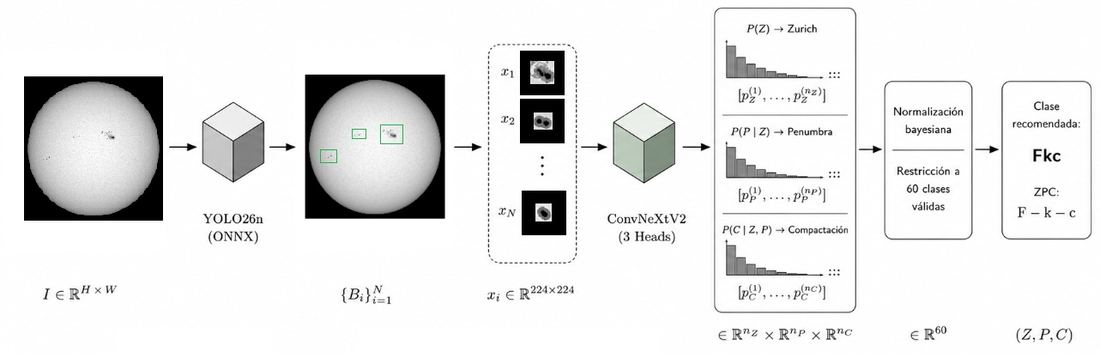
\includegraphics[width=0.98\linewidth]{figures/sys/img_pipe.jpg}
    \caption{Propuesta modular de detección y clasificación de manchas solares \textbf{Fuente:} Elaboración propia.}
    \label{fig:resumen-flujo-general}
\end{figure*}
\section{Fundamentos teóricos}

\subsection{Observaciones solares y esquema de clasificación Zurich--McIntosh}

Las manchas solares corresponden a regiones fotosféricas de menor temperatura relativa, asociadas con concentraciones intensas de campo magnético. Su número, posición y morfología varían a lo largo del ciclo solar, por lo que su registro sistemático permite estudiar tendencias temporales, asimetrías hemisféricas y fases de migración latitudinal \citep{hale1919magneticpolarity,hathaway2015solarcycle,murakozy2022asymmetries}.

La observación solar puede realizarse desde instrumentos espaciales o desde observatorios terrestres. Los primeros ofrecen continuidad y estabilidad radiométrica, mientras que los segundos permiten implementar sistemas académicos accesibles, aunque condicionados por atmósfera, enfoque, estabilidad mecánica y calidad óptica. Por ello, el trabajo adopta una estrategia complementaria entre datos de referencia, reportes NOAA SRS e imágenes capturadas localmente \citep{scherrer2012hmi,bobra2014sharp,noaaSRS,sidcGroundObservations2026}.

\begin{figure}[H]
    \centering
    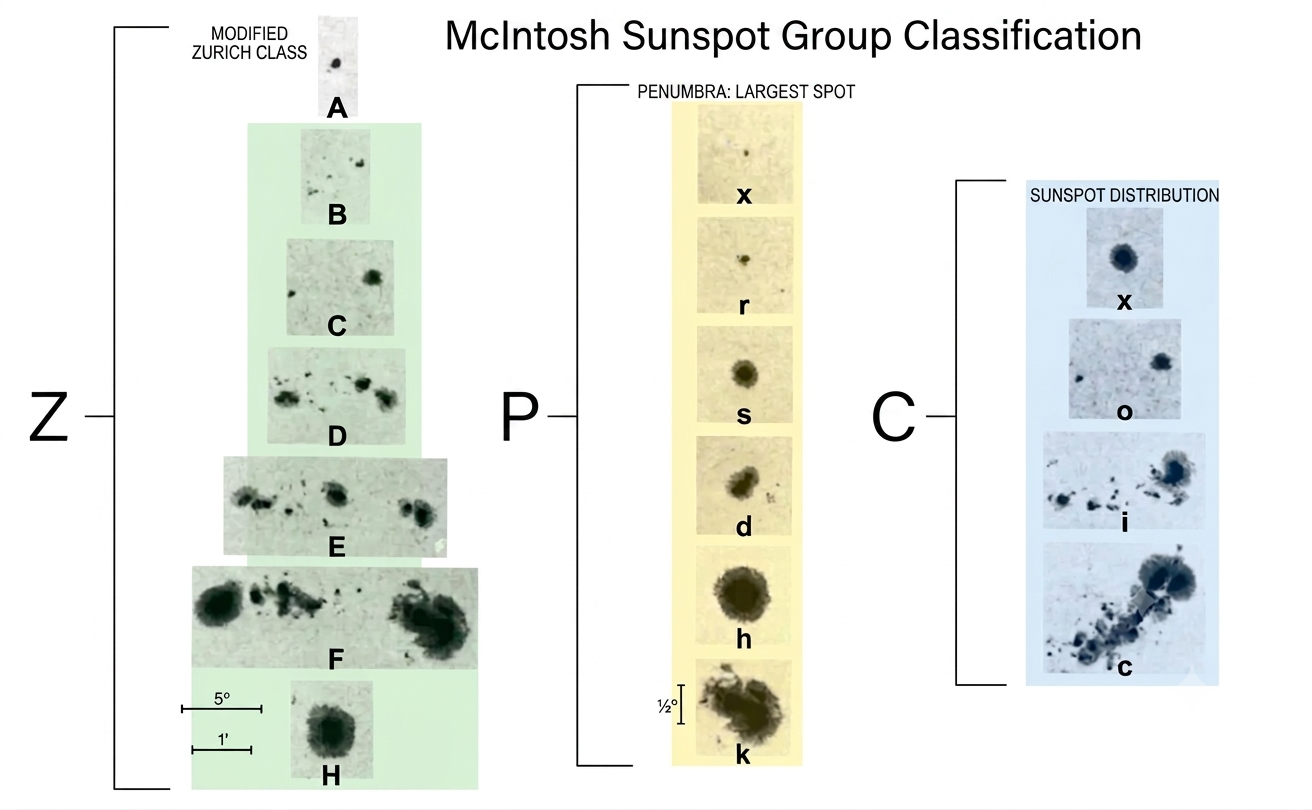
\includegraphics[width=0.7\linewidth]{figures/solar/mcintosh.png}
    \caption{Esquema de la clasificación Zurich--McIntosh utilizada para describir grupos solares. \textbf{Fuente:} Adaptado de criterios observacionales clásicos.}
    \label{fig:resumen-mcintosh}
\end{figure}

La clasificación Zurich--McIntosh describe cada grupo mediante tres componentes: clase evolutiva $Z$, tipo de penumbra $P$ y distribución interna $C$. La etiqueta final puede representarse como
\begin{equation}
    y = (Z,P,C), \qquad y \in \mathcal{Y}_{\mathrm{ZM}},
\end{equation}
donde $\mathcal{Y}_{\mathrm{ZM}}$ contiene únicamente combinaciones morfológicamente válidas. Esta formulación favorece una clasificación jerárquica, más interpretable que una clase plana de combinaciones, porque conserva la relación entre evolución global, estructura penumbral y compactación interna del grupo \citep{mcintosh1990classification,bornmann1994flarerates,watson2009wilson}.

\subsection{Agrupamiento y clasificación de manchas solares}

Los trabajos recientes sobre clasificación automática de regiones activas muestran que el aprendizaje profundo puede reproducir criterios observacionales de Mount Wilson y Zurich--McIntosh, aunque el desempeño depende de la calidad de las etiquetas, del balance entre clases y de la forma en que se incorporan restricciones físicas o taxonómicas \citep{sayez2023sunscc,zhou2023mcintosh,deng2025mcintosh}. En esta tesis se adopta, por ello, una estrategia modular: primero se agrupan y recortan regiones candidatas; luego se clasifican los recortes en los componentes $Z$, $P$ y $C$.

La primera etapa se formula como un problema de detección de objetos. Un detector de la familia YOLO estima cajas delimitadoras $b_i=(x_i,y_i,w_i,h_i)$ para cada grupo solar visible en una imagen de disco completo \citep{ultralyticsYOLO26,robUSET2026,noaaSRS,scherrer2012hmi}.

La segunda etapa recibe los recortes generados por el detector y estima la etiqueta Zurich--McIntosh. En lugar de aprender una única clase plana para cada combinación $ZPC$, el sistema emplea una arquitectura jerárquica basada en ConvNeXtV2 \citep{woo2023convnextv2,mcintosh1990classification}.

\subsection{Modelos predictivos de la actividad solar}

La predicción de la actividad solar anticipar la evolución del ciclo a partir de series históricas como el número de manchas solares, el área activa o la distribución latitudinal de los grupos, la literatura reúne enfoques de precursores físicos, modelos estadísticos de series temporales y métodos de aprendizaje automático o identificación dinámica \citep{pesnell2012predictions,clette2014revisiting,camporeale2019ml}.

Entre los métodos físicos, los precursores basados en campos polares e índices geomagnéticos ofrecen información temprana sobre la amplitud esperada de un ciclo, pero no siempre describen con detalle la evolución mensual del índice de manchas \citep{schatten2005precursor,svalgaard2005polar}. Para complementar esa limitación, la tesis incorpora un bloque PVL--Kalman que suaviza y actualiza recursivamente el número de manchas solares suavizado \citep{kalman1960newapproach,podladchikova2012kalman}.

Sin embargo, una serie escalar no conserva por sí sola la información espacial del ciclo solar. La migración de las bandas activas hacia el ecuador, visible en el diagrama de Spörer, contiene estructura física relevante para interpretar la fase del ciclo y las asimetrías latitudinales \citep{hathaway2015solarcycle,murakozy2022asymmetries}. Por ello, la tesis explora la Descomposición en Modos Dinámicos (DMD) como una línea complementaria de modelado. Cada mes se representa mediante un vector de conteos latitudinales \citep{schmid2010dmd,kutz2016dmd}.

De esta manera, PVL--Kalman aporta una predicción escalar suavizada y DMD agrega una lectura espacio-temporal de la migración latitudinal. La combinación de ambos enfoques no pretende reemplazar los pronósticos operacionales, sino proporcionar contexto físico y visual para el sistema de observación y clasificación desarrollado en la tesis \citep{podladchikova2012kalman,schmid2010dmd,kutz2016dmd}.

\section{Consideraciones de diseño}

El diseño del prototipo se organiza como un ecosistema modular desacoplado para instrumentación, recopilación, procesamiento y análisis de manchas solares. Esta separación permite asignar responsabilidades claras a cada bloque: adquisición local junto al telescopio, preprocesamiento embebido, publicación de datos, inferencia mediante modelos de aprendizaje profundo, visualización web y análisis predictivo. La arquitectura busca que cada módulo pueda validarse y actualizarse de forma independiente, sin perder la trazabilidad entre imagen original, metadatos, recortes, clasificación Zurich--McIntosh y productos de tendencia temporal \citep{raspberryPi5Docs2026,zwoASI174Manual2025,luntWhiteLightWedges2026}.

\begin{figure*}[p]
    \centering
    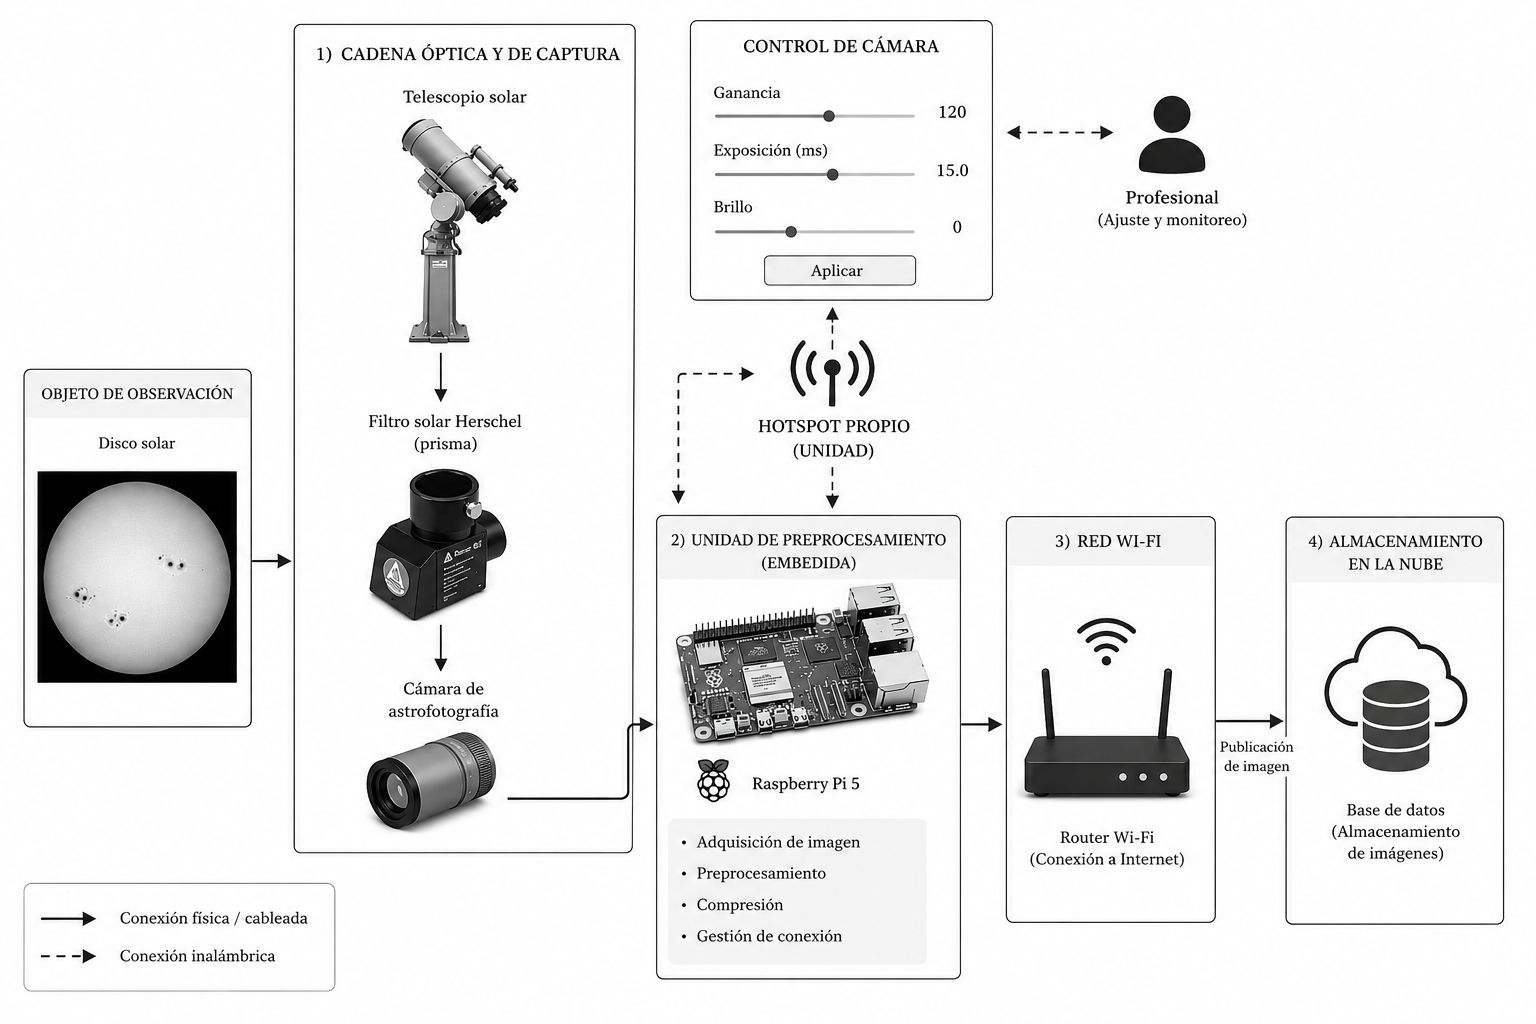
\includegraphics[height=0.38\textheight]{figures/hw/module.png}
    \caption{Flujo operativo de la etapa de preprocesamiento embebida. Se destacan la captura y calibración de imágenes de disco solar completo, la operación mediante panel web local y la publicación posterior hacia una base de datos en la nube. \textbf{Fuente:} Elaboración propia.}
    \label{fig:resumen-flujo-preprocesamiento-embebido}

    \vspace{0.25em}
    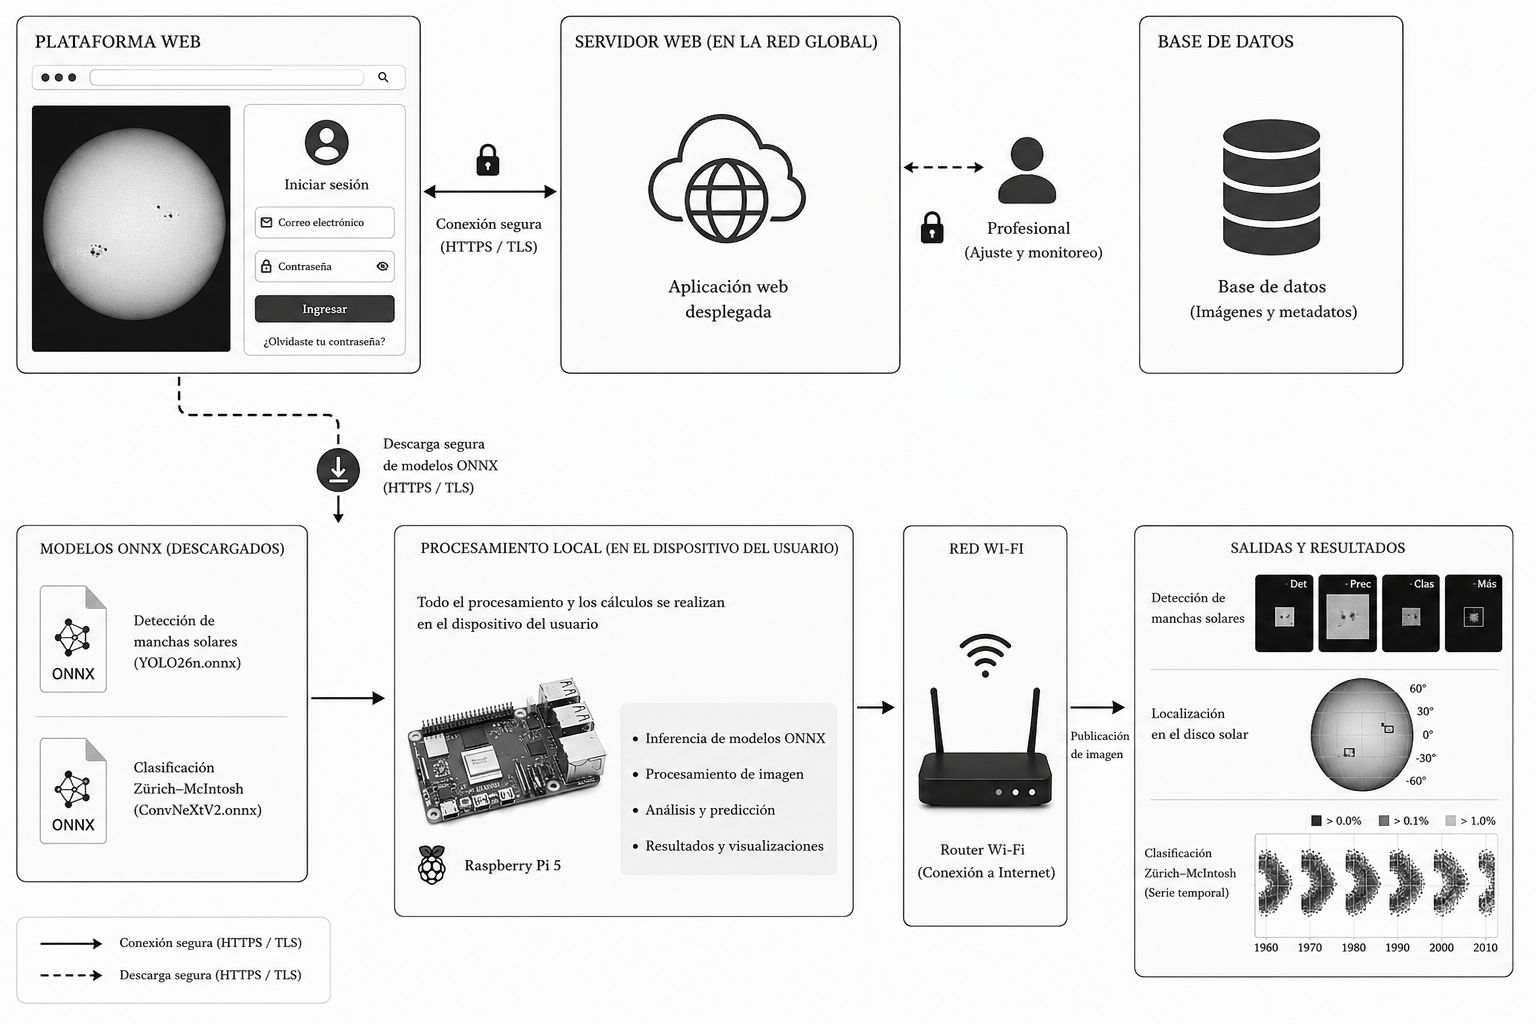
\includegraphics[height=0.38\textheight]{figures/hw/camera_mount.png}
    \caption{Flujo operativo de procesamiento, agrupamiento, clasificación ONNX y análisis predictivo de actividad solar. \textbf{Fuente:} Elaboración propia.}
    \label{fig:resumen-flujo-procesamiento-onnx}
\end{figure*}

Las Figuras~\ref{fig:resumen-flujo-preprocesamiento-embebido} y~\ref{fig:resumen-flujo-procesamiento-onnx} resumen las dos capas principales del flujo de trabajo. La primera corresponde a la unidad embebida que funciona junto al tren óptico y cumple una función dual de conectividad: puede generar una red WiFi local para configuración directa en campo o conectarse como cliente a una red disponible para sincronizar datos. Desde este nodo se controlan la calibración, la captura de imágenes de disco completo y los ajustes de exposición, ganancia y saturación. El panel web local evita depender de una estación externa permanente y permite supervisar el estado del dispositivo durante la observación.

La cámara seleccionada fue la ZWO ASI174MM Mini, principalmente por su sensor monocromático IMX174, obturador global, píxel de $5.86\,\mu\mathrm{m}$ y formato compacto. Estas características son relevantes para capturar estructuras fotosféricas con baja distorsión temporal y buen acoplamiento al tren óptico de observación solar \citep{zwoASI174Manual2025,sonyPregiusGlobalShutter,zwoGuideCameras2025}.

Una vez preprocesadas, las observaciones se publican en una base de datos que actúa como repositorio intermedio de imágenes, metadatos y registros observacionales. Esta decisión desacopla la captura de las etapas posteriores: la plataforma web puede consultar los datos disponibles, ejecutar modelos ONNX para agrupamiento y clasificación, presentar tendencias de actividad y conservar registros del Observatorio Astronómico ``Prof. Alexis Troche Boggino''. Así, el flujo no termina en la captura, sino que continúa hacia una capa abierta de análisis y consulta. La segunda capa integra la localización de grupos solares, la clasificación Zurich--McIntosh y la generación de contexto predictivo, manteniendo una cadena continua desde la instrumentación solar hasta la interpretación científica de los resultados.

\begin{figure*}[t]
    \centering
    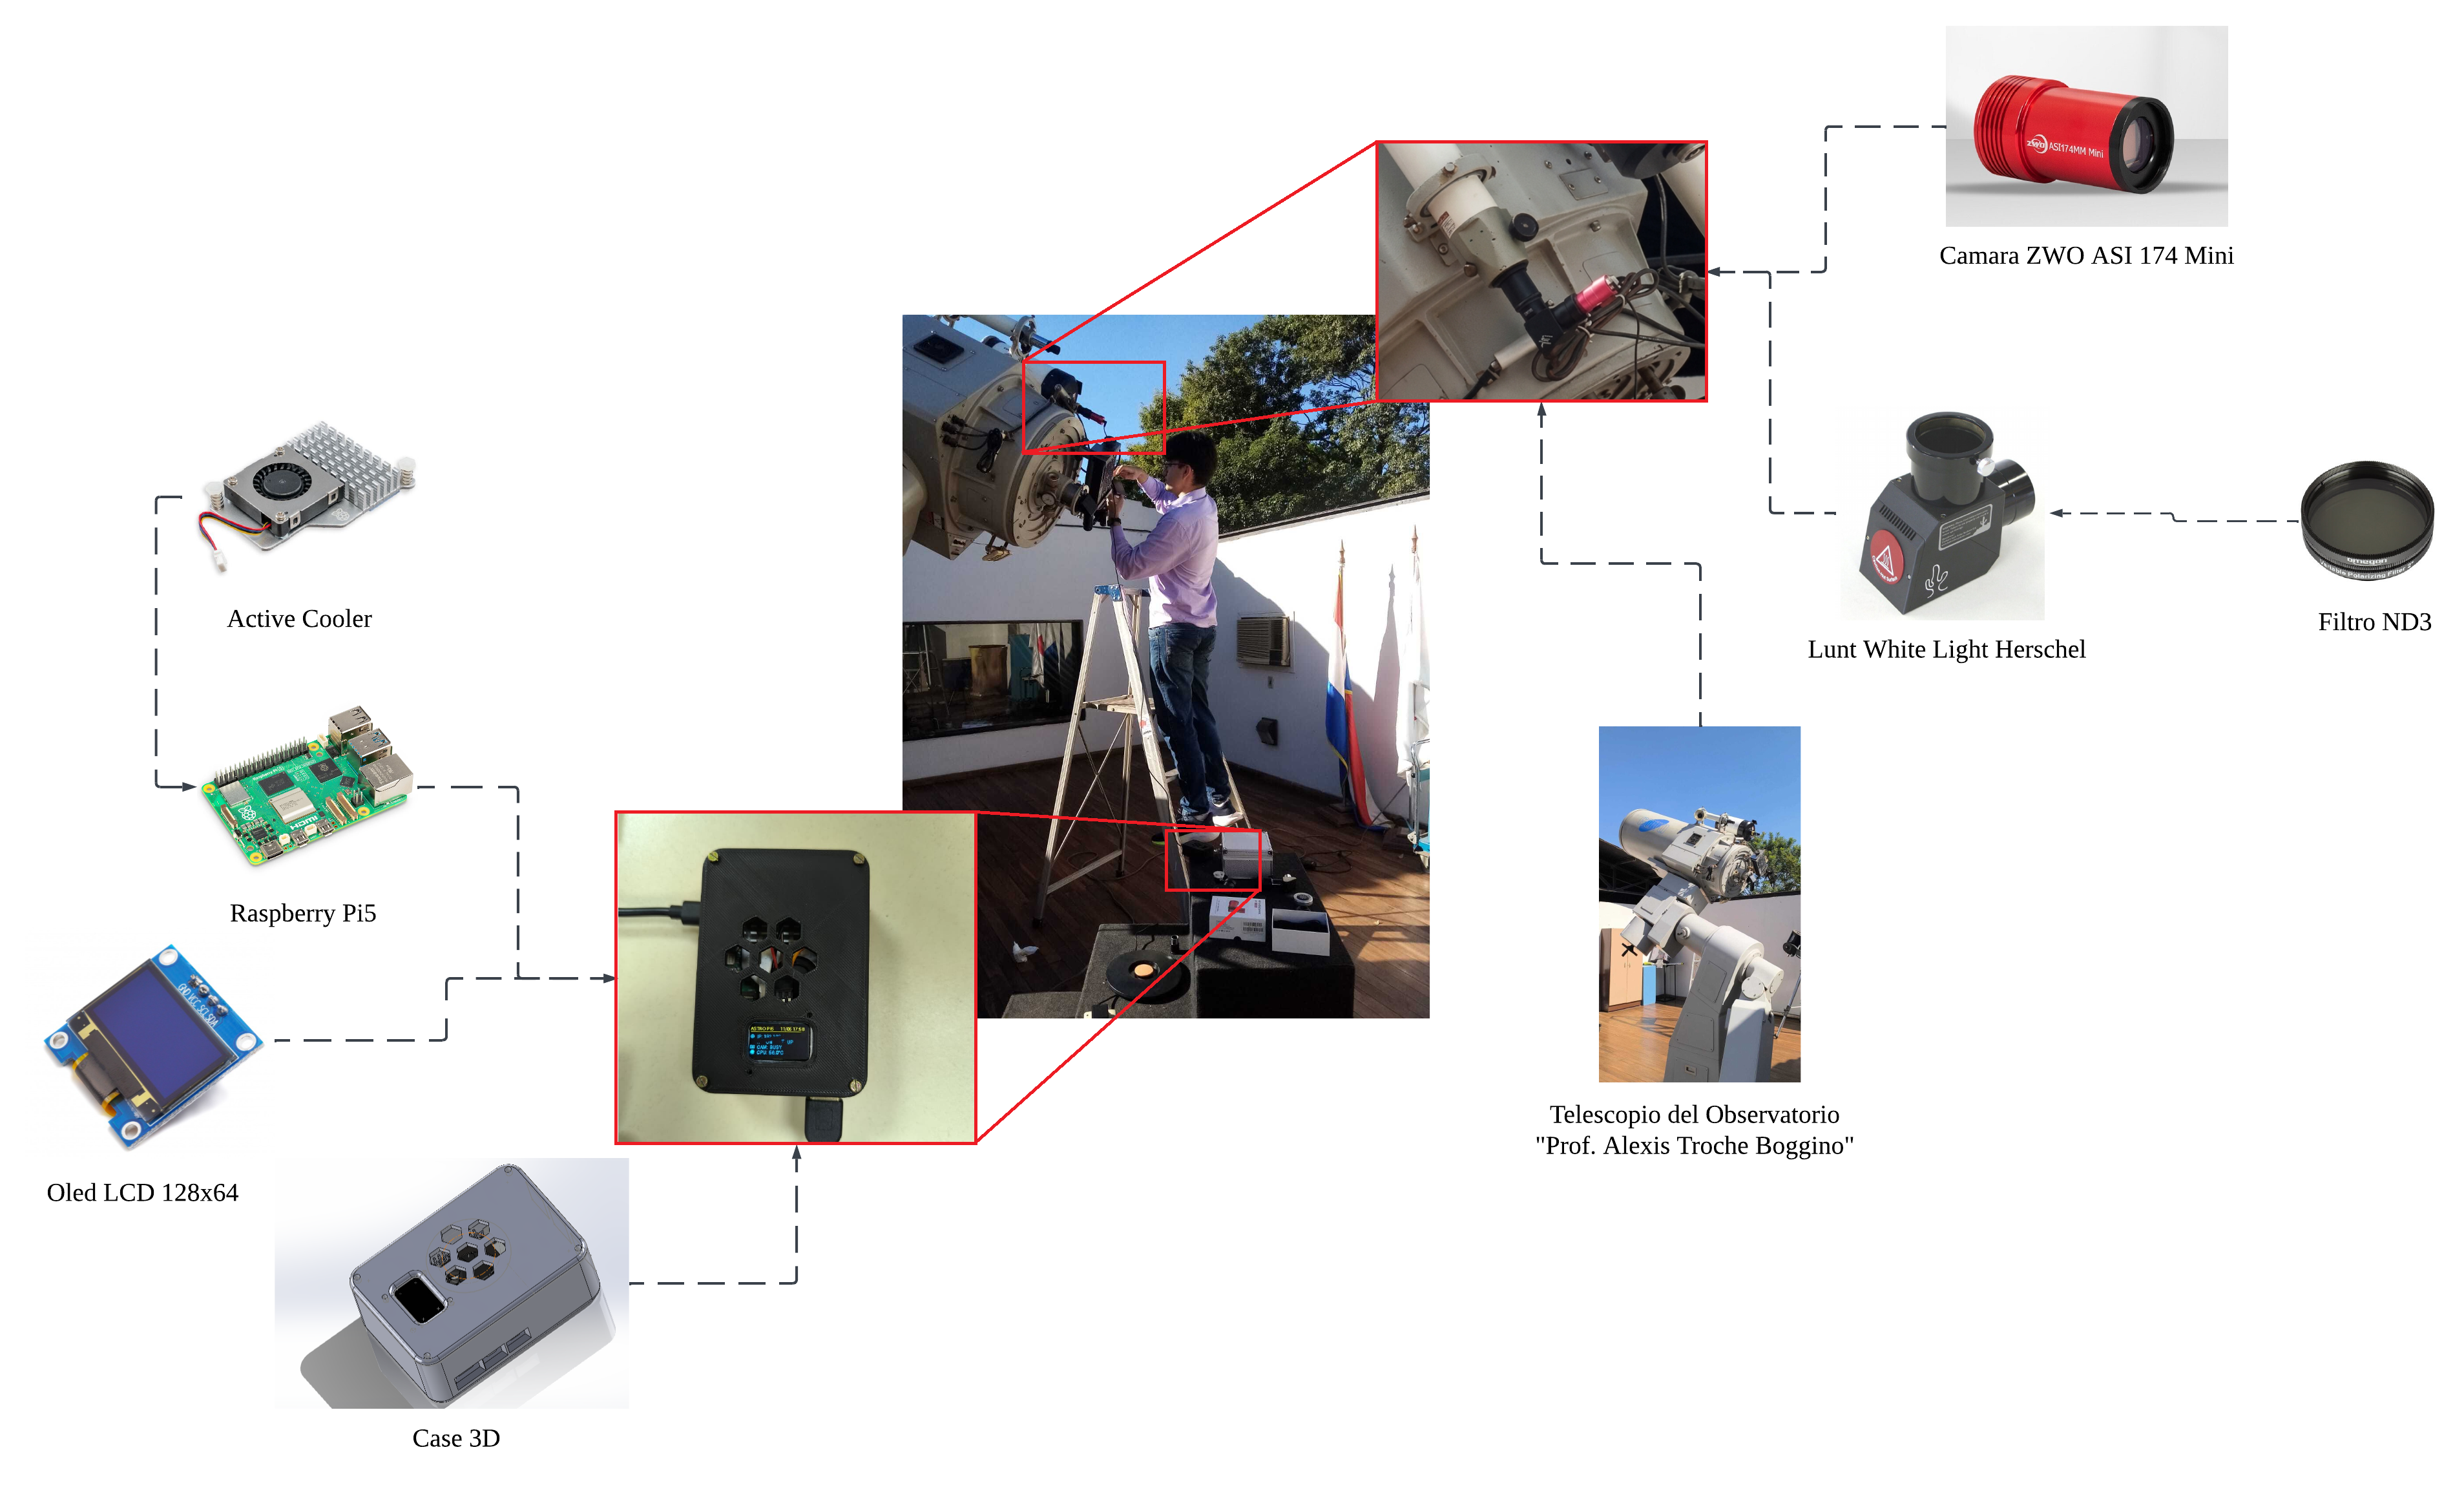
\includegraphics[width=0.9\linewidth]{figures/hw/hw_diagram.png}
    \caption{Componentes del flujo de adquisición de la imagen. \textbf{Fuente:} Elaboración propia.}
    \label{fig:resumen-componentes-adquisicion}
\end{figure*}

En cuanto a la cadena de procesamiento integrada en los modelos de aprendizaje profundo, se define como un modelo en cascada. Primero, el detector estima cajas $b_i=(x_i,y_i,w_i,h_i)$ para grupos solares; luego, cada recorte alimenta un clasificador jerárquico que estima probabilidades $p(Z\mid I)$, $p(P\mid Z,I)$ y $p(C\mid Z,P,I)$. La probabilidad conjunta se expresa como
\begin{equation}
    p(Z,P,C\mid I)=p(Z\mid I)\,p(P\mid Z,I)\,p(C\mid Z,P,I),
\end{equation}
lo que permite ordenar recomendaciones y descartar combinaciones no válidas \citep{mcintosh1990classification,woo2023convnextv2,cui2019classbalanced}.

Para el análisis predictivo se combinan dos representaciones: una escalar para el número de manchas solares y otra espacio-temporal para el diagrama de Spörer. En el modelo PVL--Kalman, la transición mensual se ajusta mediante un factor $\Phi_k$ y se corrige con la ganancia de Kalman $K_k$, mientras que DMD aproxima la evolución latitudinal mediante $\mathbf{x}_{k+1}\approx\mathbf{A}\mathbf{x}_k$ \citep{podladchikova2012kalman,kalman1960newapproach,schmid2010dmd,kutz2016dmd}.

\section{Diseño del hardware}

El hardware se estructura en una unidad de procesamiento embebido basada en Raspberry Pi 5, encargada de adquisición, preprocesamiento, comunicación local y soporte de interacción. La elección responde a su disponibilidad, capacidad de cómputo, soporte de periféricos y facilidad de integración en un módulo portátil de observación \citep{raspberryPi5Docs2026,nmcliHotspot2026}.


El sistema de captura integra la cámara monocromática, el tren óptico de observación en luz blanca y la cuña de Herschel como elemento de atenuación segura. Esta configuración busca preservar contraste en umbra y penumbra, evitar saturación y mantener condiciones compatibles con el procesamiento automático posterior \citep{zwoASI174Manual2025,luntWhiteLightWedges2026,baaderHerschelUsage2026}.

La unidad local incorpora visualización de estado y conectividad de red para facilitar operación en campo. La pantalla OLED se conecta mediante una interfaz I2C simple. Esta decisión reduce dependencia de una consola externa durante tareas de captura y verificación \citep{raspberryPi5Docs2026,nmcliHotspot2026}.

La carcasa y los soportes impresos en 3D cumplen una función operativa: protegen el nodo de procesamiento, ordenan el cableado, permiten ventilación y facilitan el montaje en campañas observacionales. El resultado es una estación compacta que puede operar como módulo de adquisición en observatorios locales \citep{raspberryPi5Docs2026,zwoASILinuxManual}.



\section{Diseño del software}

El software articula datos, entrenamiento, almacenamiento, despliegue e interfaz web. La base de datos de entrenamiento se construye vinculando imágenes heliográficas con reportes observacionales, de modo que las etiquetas Zurich--McIntosh y los metadatos temporales puedan usarse para entrenar y auditar modelos de detección y clasificación \citep{noaaSRS,scherrer2012hmi,bobra2014sharp,robUSET2026}.

\subsection{Obtención y preparación de datos}

Los datos se obtuvieron acoplando imágenes fotosféricas SDO/HMI de disco completo con reportes diarios NOAA SRD/SRS para el período 2010--2025. DB1 conserva el disco completo con cajas de grupos solares obtenidas a partir de proyecciones heliográficas y filtros como el \textit{black-hat}; DB2 contiene recortes normalizados de $224\times224$; y DB2.1 refina esos recortes mediante detecciones YOLO26n y realce morfológico para mejorar la correspondencia entre imagen, posición y etiqueta \citep{scherrer2012hmi,noaaSRS,cesarHeliographic,robUSET2026}.

\begin{table}[H]
\centering
\caption{Resumen de bases de datos utilizadas para entrenamiento y refinamiento. \textbf{Fuente:} Elaboración propia a partir del flujo de construcción de datos.}
\label{tab:resumen-bases-datos}
%\scriptsize
\begin{tabular}{lp{0.25\linewidth}cp{0.30\linewidth}}
\toprule
\textbf{Base} & \textbf{Observación} & \textbf{Registros} & \textbf{Uso principal} \\
\midrule
DB1 & Disco completo & $\sim$4700 & Entrenamiento de YOLO26n \\
DB2 & Grupo solar & $\sim$15000 & Etapa intermedia \\
DB2.1 & Grupo solar refinado (Yolo26n+PCA) & $\sim$14300 & Entrenamiento de ConvNeXtV2a \\
\bottomrule
\end{tabular}
\end{table}

\subsection{Detección de grupos solares}

El detector YOLO26n localiza grupos solares y produce recortes que reducen el dominio visual para la clasificación; las curvas de pérdida, precisión, \textit{recall} y mAP permiten verificar la convergencia del detector y su utilidad para construir recortes consistentes \citep{ultralyticsYOLO26,robUSET2026,noaaSRS}.

\begin{figure}[H]
    \centering
    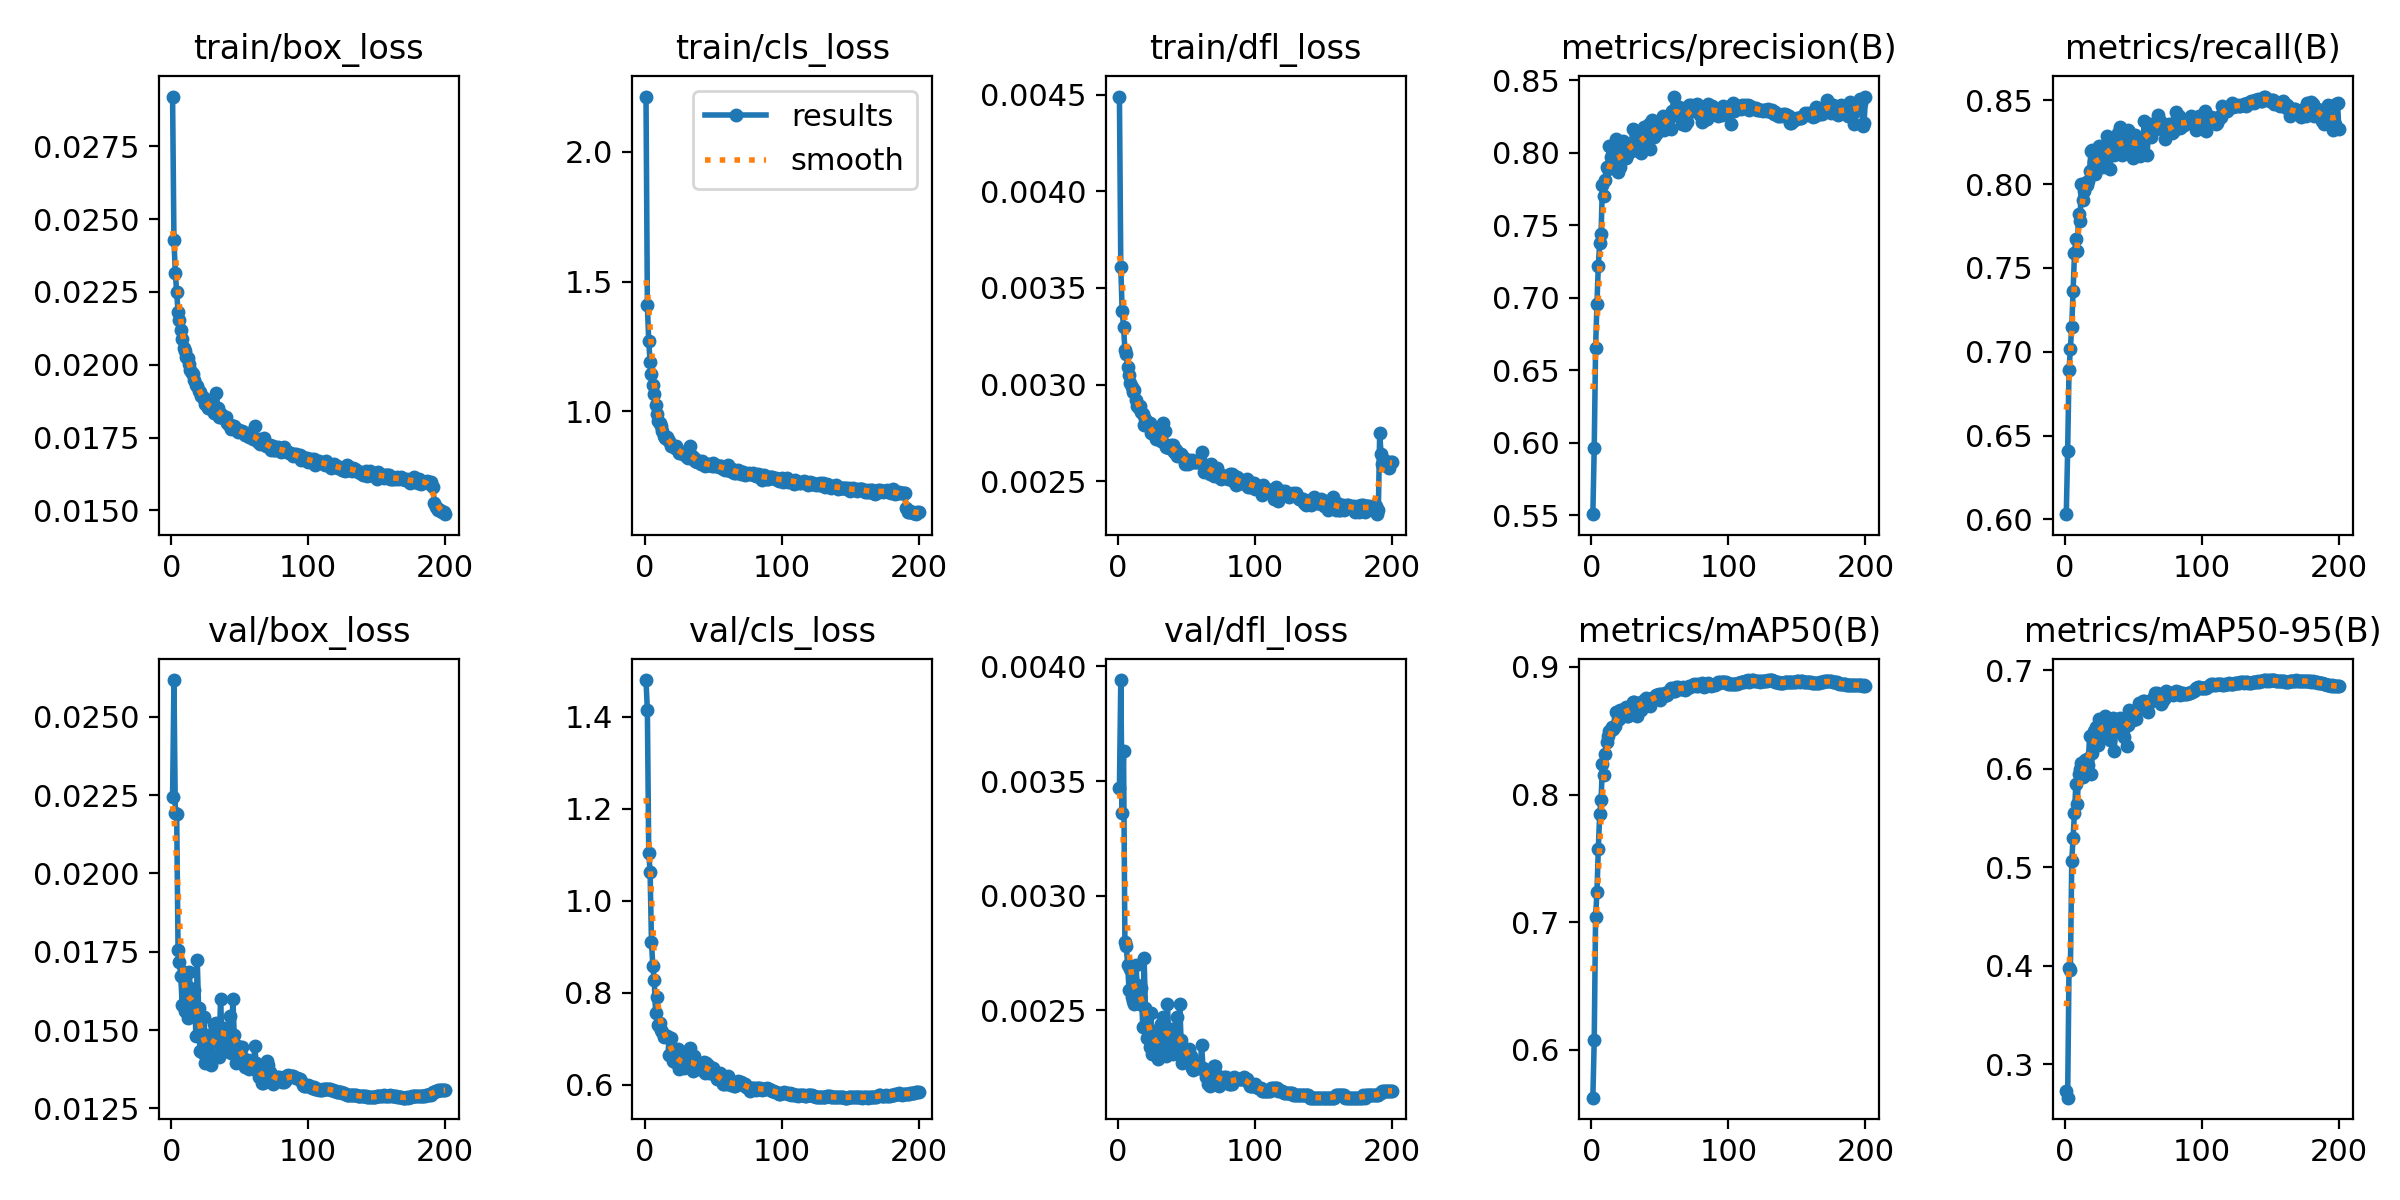
\includegraphics[width=0.92\linewidth]{figures/ml/yolo_results.png}
    \caption{Métricas de entrenamiento del detector YOLO26n sobre DB1, incluyendo pérdidas de entrenamiento/validación, precisión, \textit{recall} y mAP. \textbf{Fuente:} Elaboración propia.}
    \label{fig:resumen-yolo-training}
\end{figure}

\subsection{Clasificación jerárquica Zurich--McIntosh}

Luego, ConvNeXtV2 Atto opera como extractor compacto de características para los recortes normalizados de regiones activas. Esta división separa localización y descripción morfológica, reduce la complejidad frente a una clase plana $ZPC$ y preserva la interpretación astronómica de cada salida \citep{woo2023convnextv2,mcintosh1990classification,zhou2023mcintosh}.

\begin{figure*}[t]
    \centering
    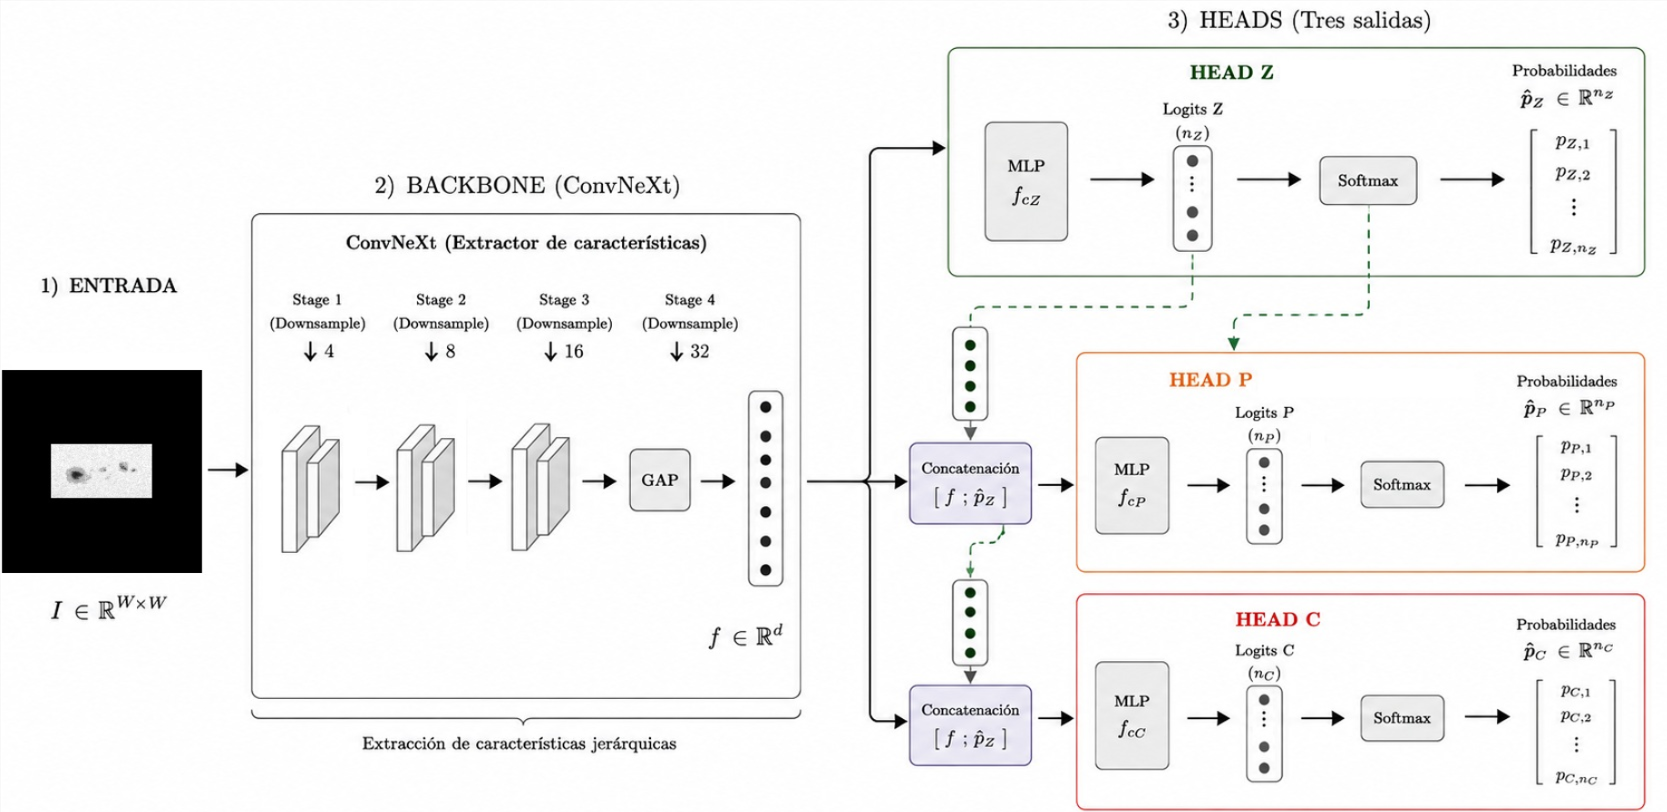
\includegraphics[width=0.98\textwidth]{figures/ml/convnext_arch.png}
    \caption{Arquitectura de clasificación jerárquica basada en ConvNeXtV2 para componentes Zurich--McIntosh. El recorte solar se transforma mediante el extractor ConvNeXtV2; luego, el agrupamiento promedio global produce el vector latente $\mathbf{f}$, a partir del cual se calcula primero la distribución $\hat{\mathbf{p}}_Z$. Las salidas $P$ y $C$ usan la concatenación $[\mathbf{f};\hat{\mathbf{p}}_Z]$ para incorporar dependencia jerárquica antes de la recomendación final. \textbf{Fuente:} Elaboración propia con base en ConvNeXtV2.}
    \label{fig:resumen-convnext}
\end{figure*}

La Figura~\ref{fig:resumen-convnext} resume el flujo jerárquico del clasificador. Para un recorte $x\in\mathbb{R}^{224\times224}$, el backbone ConvNeXtV2 produce mapas de características que se resumen mediante agrupamiento promedio global en un vector
\begin{equation}
\mathbf{f}=\operatorname{GAP}(\operatorname{ConvNeXtV2}(x)), \qquad \mathbf{f}\in\mathbb{R}^{d}.
\end{equation}
La primera salida estima la distribución del carácter Zurich,
\begin{equation}
\hat{\mathbf{p}}_Z=\operatorname{softmax}(g_Z(\mathbf{f})), \qquad \hat{\mathbf{p}}_Z\in\mathbb{R}^{n_Z}.
\end{equation}
Luego, las salidas penumbral y de compactación incorporan la dependencia con $Z$ usando la concatenación del vector visual y la distribución Zurich:
\begin{equation}
\hat{\mathbf{p}}_P=\operatorname{softmax}(g_P([\mathbf{f};\hat{\mathbf{p}}_Z])), \qquad
\hat{\mathbf{p}}_C=\operatorname{softmax}(g_C([\mathbf{f};\hat{\mathbf{p}}_Z])).
\end{equation}
Por tanto, el clasificador se expresa como
\begin{equation}
f_\theta(x)=\left(\hat{\mathbf{p}}_Z,\hat{\mathbf{p}}_P,\hat{\mathbf{p}}_C\right),
\end{equation}
donde cada término es una distribución probabilística sobre una componente de la taxonomía. Esta formulación conserva la estructura semántica Zurich--McIntosh y facilita la exportación del modelo a ONNX como un sistema multisalida \citep{woo2023convnextv2,mcintosh1990classification}.

\subsection{Posprocesamiento probabilístico}

El posprocesamiento convierte las tres salidas del clasificador en una recomendación probabilística restringida al espacio válido de clases Zurich--McIntosh. Para una imagen $x$, la probabilidad conjunta ideal se expresa como
\begin{equation}
P(Z,P,C\mid x)=P(Z\mid x)P(P\mid Z,x)P(C\mid Z,P,x).
\end{equation}
Como implementación operativa se usa una base factorizada,
\begin{equation}
P_{\mathrm{base}}(Z,P,C\mid x)=P(Z\mid x)P(P\mid x)P(C\mid x),
\end{equation}
y se aplica una máscara binaria $M_{ZPC}$ para anular combinaciones no admisibles. La distribución recomendada queda normalizada como
\begin{equation}
P_{\mathrm{rec}}(Z,P,C\mid x)=
\frac{P_{\mathrm{base}}(Z,P,C\mid x)M_{ZPC}}
{\sum_{z,p,c}P_{\mathrm{base}}(z,p,c\mid x)M_{zpc}}.
\end{equation}
La clase final se obtiene con $(Z^\ast,P^\ast,C^\ast)=\arg\max_{Z,P,C}P_{\mathrm{rec}}(Z,P,C\mid x)$, manteniendo interpretabilidad y consistencia taxonómica \citep{mcintosh1990classification,sayez2023sunscc}.

\subsection{Modelos predictivos}

Para los modelos predictivos, el número de manchas solares suavizado se estima con PVL--Kalman. La etapa de actualización queda dada por
\begin{equation}
K_k=P_k^{-}(P_k^{-}+R_k)^{-1}, \qquad
\widehat{s}_k=\widehat{s}_k^{-}+K_k(z_k-\widehat{s}_k^{-}),
\end{equation}
donde $z_k$ es la observación mensual y $\widehat{s}_k$ la estimación corregida. Este bloque resume la amplitud temporal del ciclo solar mediante una serie escalar \citep{kalman1960newapproach,podladchikova2012kalman}.

El modelo DMD complementa esa salida escalar con una reconstrucción de la distribución latitudinal de actividad. Cada observación mensual se transforma en un vector de conteos latitudinales. Sea $N_{\mathrm{spots}}(t)$ el número total de manchas en el instante $t$ y $\theta_i(t)$ la latitud heliográfica de la $i$-ésima mancha; el dominio se restringe a
\begin{equation}
\theta\in[-50^{\circ},50^{\circ}], \qquad \Delta\theta=4^{\circ}, \qquad M=25.
\end{equation}
El $j$-ésimo contenedor se define como $\mathcal{B}_j=[\theta_j,\theta_{j+1})$ y su conteo como
\begin{equation}
V_j(t)=\sum_{i=1}^{N_{\mathrm{spots}}(t)}\Psi_{j,i}(t), \qquad
\Psi_{j,i}(t)=
\begin{cases}
1, & \theta_i(t)\in\mathcal{B}_j,\\
0, & \theta_i(t)\notin\mathcal{B}_j,
\end{cases}
\end{equation}
de modo que $\Psi_{j,i}(t)$ actúa como función indicadora de pertenencia de la mancha $i$ al contenedor latitudinal $j$.
Con ello, el estado latitudinal mensual queda dado por
\begin{equation}
\mathbf{x}_t=\begin{bmatrix}V_1(t)&V_2(t)&\cdots&V_M(t)\end{bmatrix}^{T}\in\mathbb{R}^{M},
\end{equation}
y la secuencia histórica se organiza como matriz de instantáneas:
\begin{equation}
\mathbf{X}=\begin{bmatrix}\mathbf{x}_1&\mathbf{x}_2&\cdots&\mathbf{x}_N\end{bmatrix}\in\mathbb{R}^{M\times N}.
\end{equation}

La Descomposición en Modos Dinámicos aproxima la evolución mediante un operador lineal efectivo $\mathbf{A}$, de modo que
\begin{equation}
\mathbf{x}_{k+1}\approx\mathbf{A}\mathbf{x}_{k}.
\end{equation}
A partir de $\mathbf{X}$ se construyen matrices desplazadas de estados consecutivos:
\begin{equation}
\mathbf{X}_1=\begin{bmatrix}\mathbf{x}_1&\cdots&\mathbf{x}_{N-1}\end{bmatrix},\quad
\mathbf{X}_2=\begin{bmatrix}\mathbf{x}_2&\cdots&\mathbf{x}_{N}\end{bmatrix}.
\end{equation}
El operador se estima con una SVD truncada de rango $r=10$,
\begin{equation}
\mathbf{X}_1\approx\mathbf{U}_r\boldsymbol{\Sigma}_r\mathbf{V}_r^{H},
\end{equation}
y se reconstruye como
\begin{equation}
\mathbf{A}\approx\mathbf{X}_2\mathbf{V}_r\boldsymbol{\Sigma}_r^{-1}\mathbf{U}_r^{H}.
\end{equation}
La proyección futura se calcula iterativamente mediante
\begin{equation}
\widehat{\mathbf{x}}_{k+1}=\mathbf{A}\widehat{\mathbf{x}}_k, \qquad k>N.
\end{equation}
Finalmente, el índice global derivado de DMD se obtiene integrando la distribución latitudinal predicha:
\begin{equation}
\widehat{\mathbf{x}}_t=\begin{bmatrix}\widehat{V}_1(t)&\widehat{V}_2(t)&\cdots&\widehat{V}_M(t)\end{bmatrix}^{T},
\end{equation}
\begin{equation}
\mathrm{SSN}_{\mathrm{DMD}}(t)=\kappa\sum_{j=1}^{M}\widehat{V}_j(t), \qquad
\kappa=\frac{\sum_{t=1}^{N}\mathrm{SSN}_{\mathrm{obs}}(t)}{\sum_{t=1}^{N}\sum_{j=1}^{M}\widehat{V}_j(t)}.
\end{equation}
Estas ecuaciones permiten pasar de una representación latitudinal física a una magnitud comparable con el SSN histórico, sin perder la lectura espacio-temporal del diagrama de Spörer \citep{schmid2010dmd,kutz2016dmd,hathaway2015solarcycle}.

\subsection{Plataforma web e inferencia portable}

La plataforma web se implementa con una lógica de consulta, visualización e inferencia portable. La conversión de modelos a ONNX permite ejecutar inferencia en entornos locales o de navegador, disminuyendo dependencia de un servidor central y facilitando uso en condiciones de conectividad limitada \citep{woo2023convnextv2,ultralyticsYOLO26,camporeale2019ml}.
\section{Resultados y validación}

\subsection{Resultados experimentales}

Los resultados experimentales confirman que la separación entre detección y clasificación es adecuada. El detector YOLO26n localiza grupos solares y genera recortes para la etapa morfológica.\citep{ultralyticsYOLO26,mcintosh1990classification,palladino2022sunspot}.

El clasificador jerárquico conserva salidas separadas para $Z$, $P$ y $C$, con un F1 promedio cercano a los mejores valores de referencia considerados. Esta decisión evita compactar artificialmente clases raras y ofrece al usuario probabilidades y alternativas plausibles, en lugar de una única etiqueta opaca \citep{sayez2023sunscc,deng2025mcintosh,woo2023convnextv2}.

\begin{figure}[H]
    \centering
    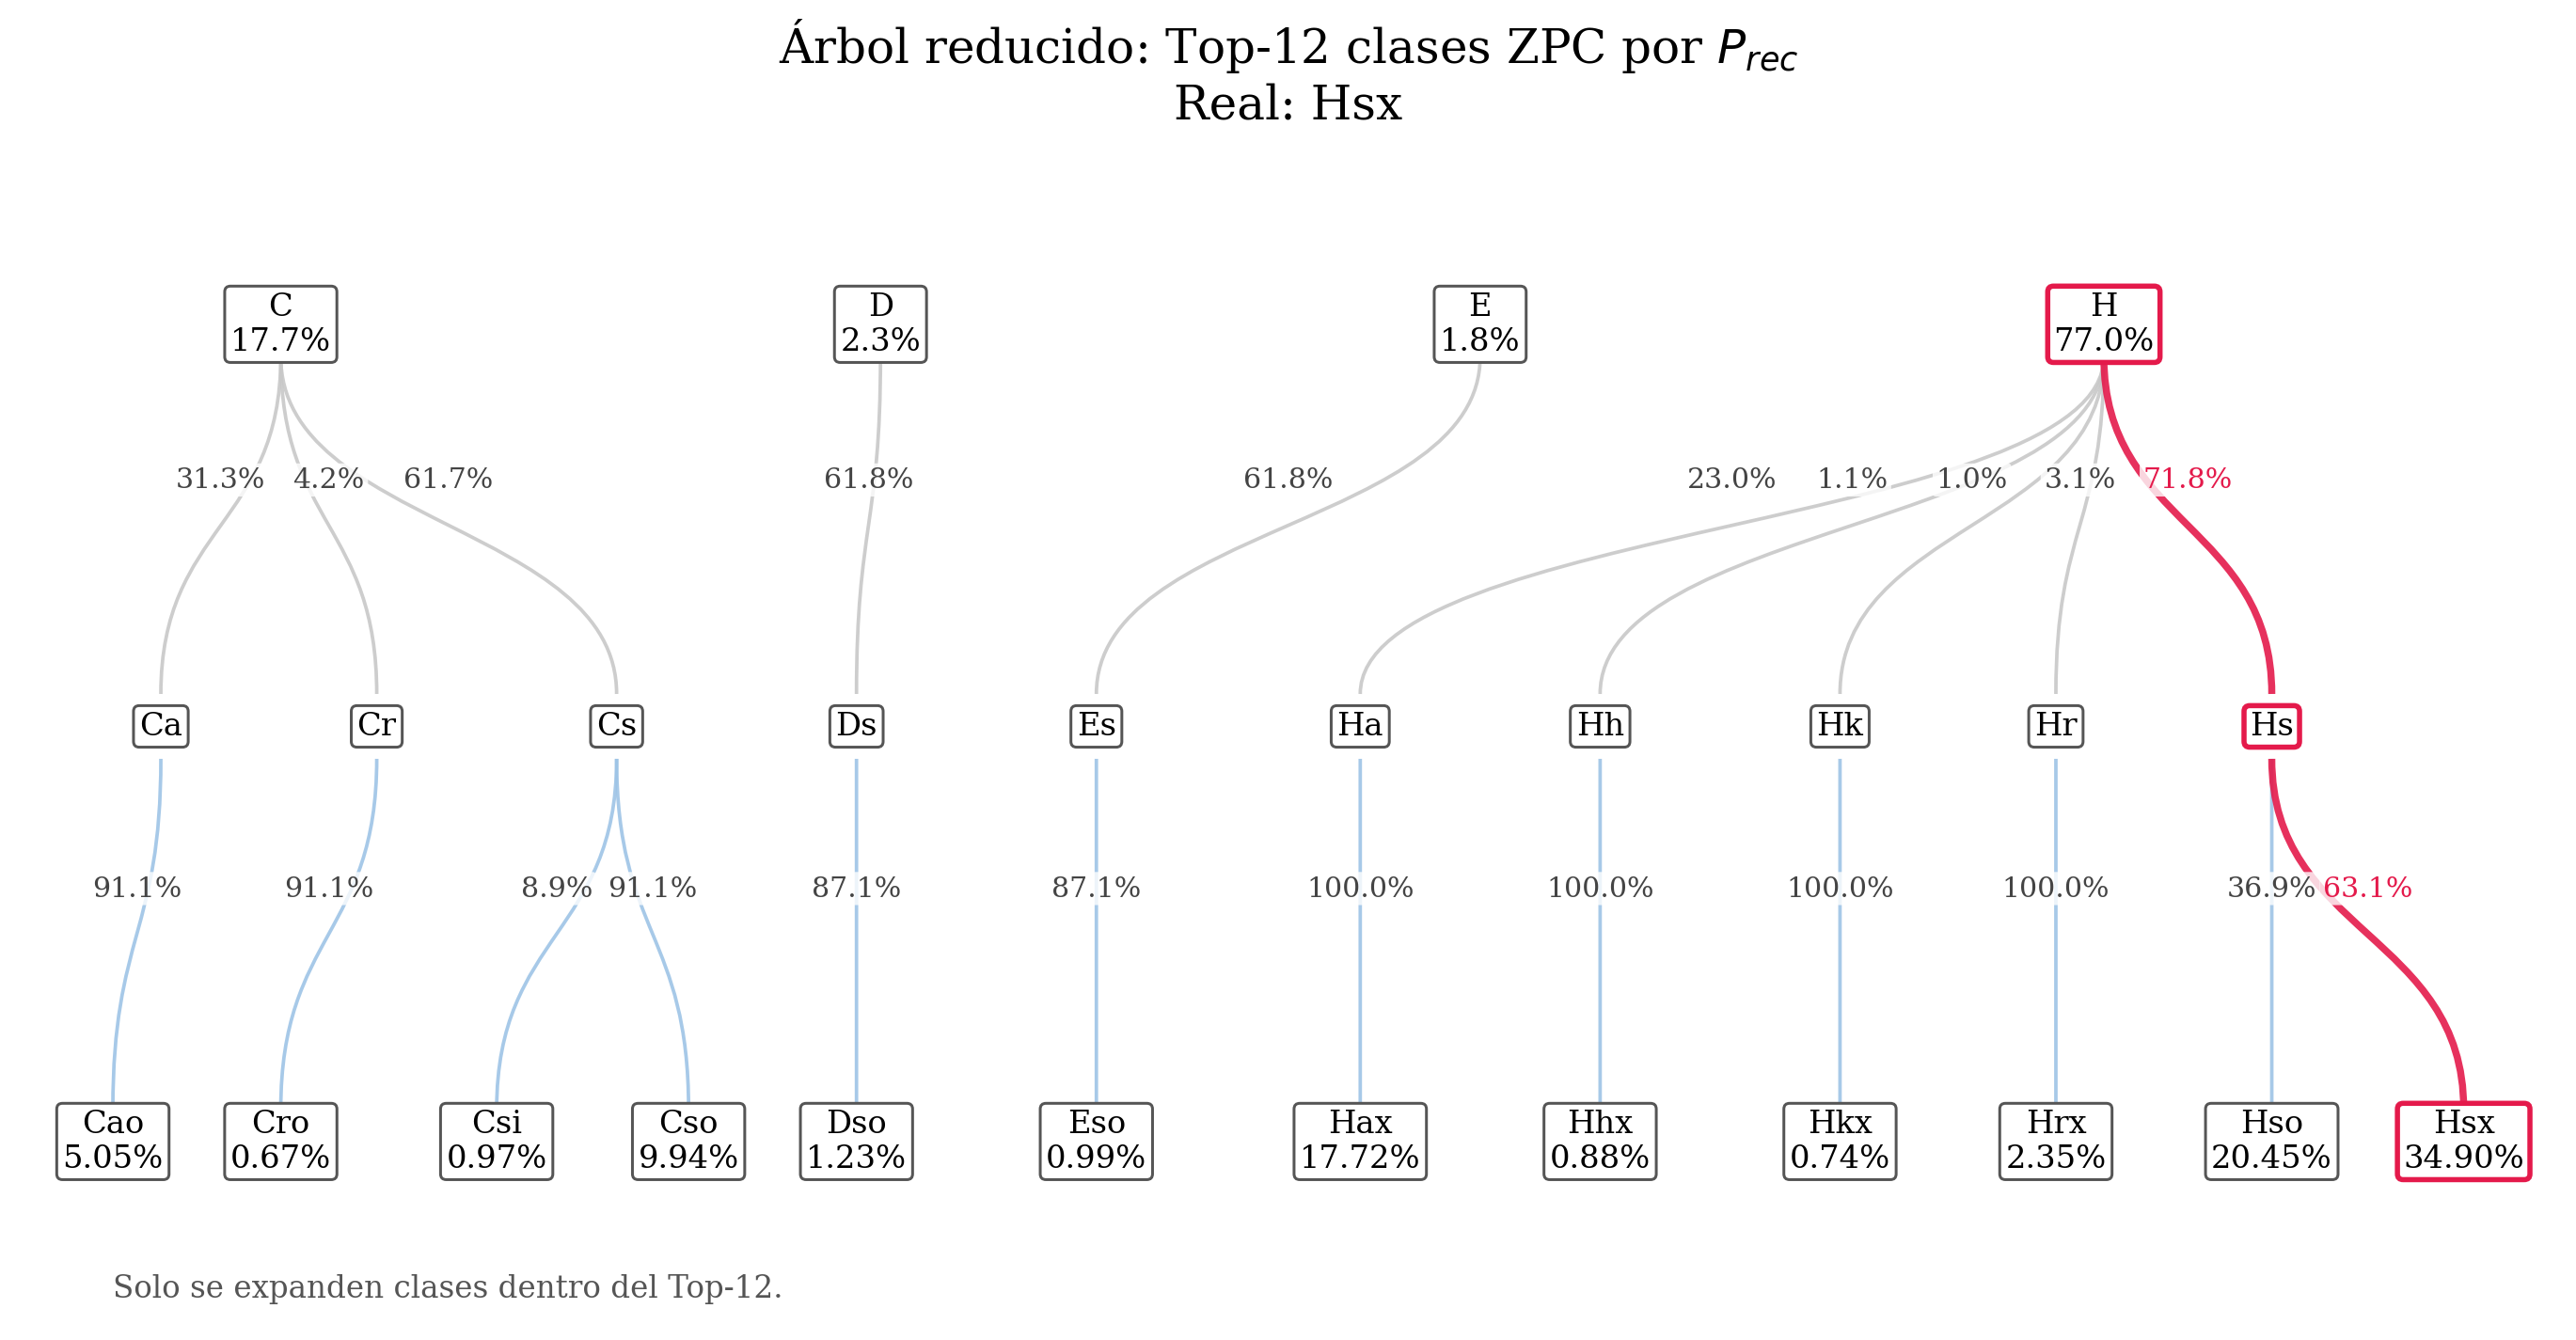
\includegraphics[width=0.92\linewidth]{figures/ml/top12_tree.png}
    \caption{Árbol bayesiano de probabilidades para la recomendación jerárquica Zurich--McIntosh. La visualización organiza alternativas probables según $Z$, $P$ y $C$, preservando consistencia taxonómica. \textbf{Fuente:} Elaboración propia.}
    \label{fig:resumen-arbol-probabilidades}
\end{figure}

El árbol de probabilidades implementa la distribución $P_{\mathrm{rec}}(Z,P,C\mid x)$ definida en el diseño del software. Esta representación permite inspeccionar cómo se reparte la confianza desde el tipo de grupo hacia las componentes penumbrales y de compactación, lo que resulta útil cuando varias configuraciones morfológicas son cercanas \citep{mcintosh1990classification,bornmann1994flarerates}.

\begin{figure}[H]
    \centering
    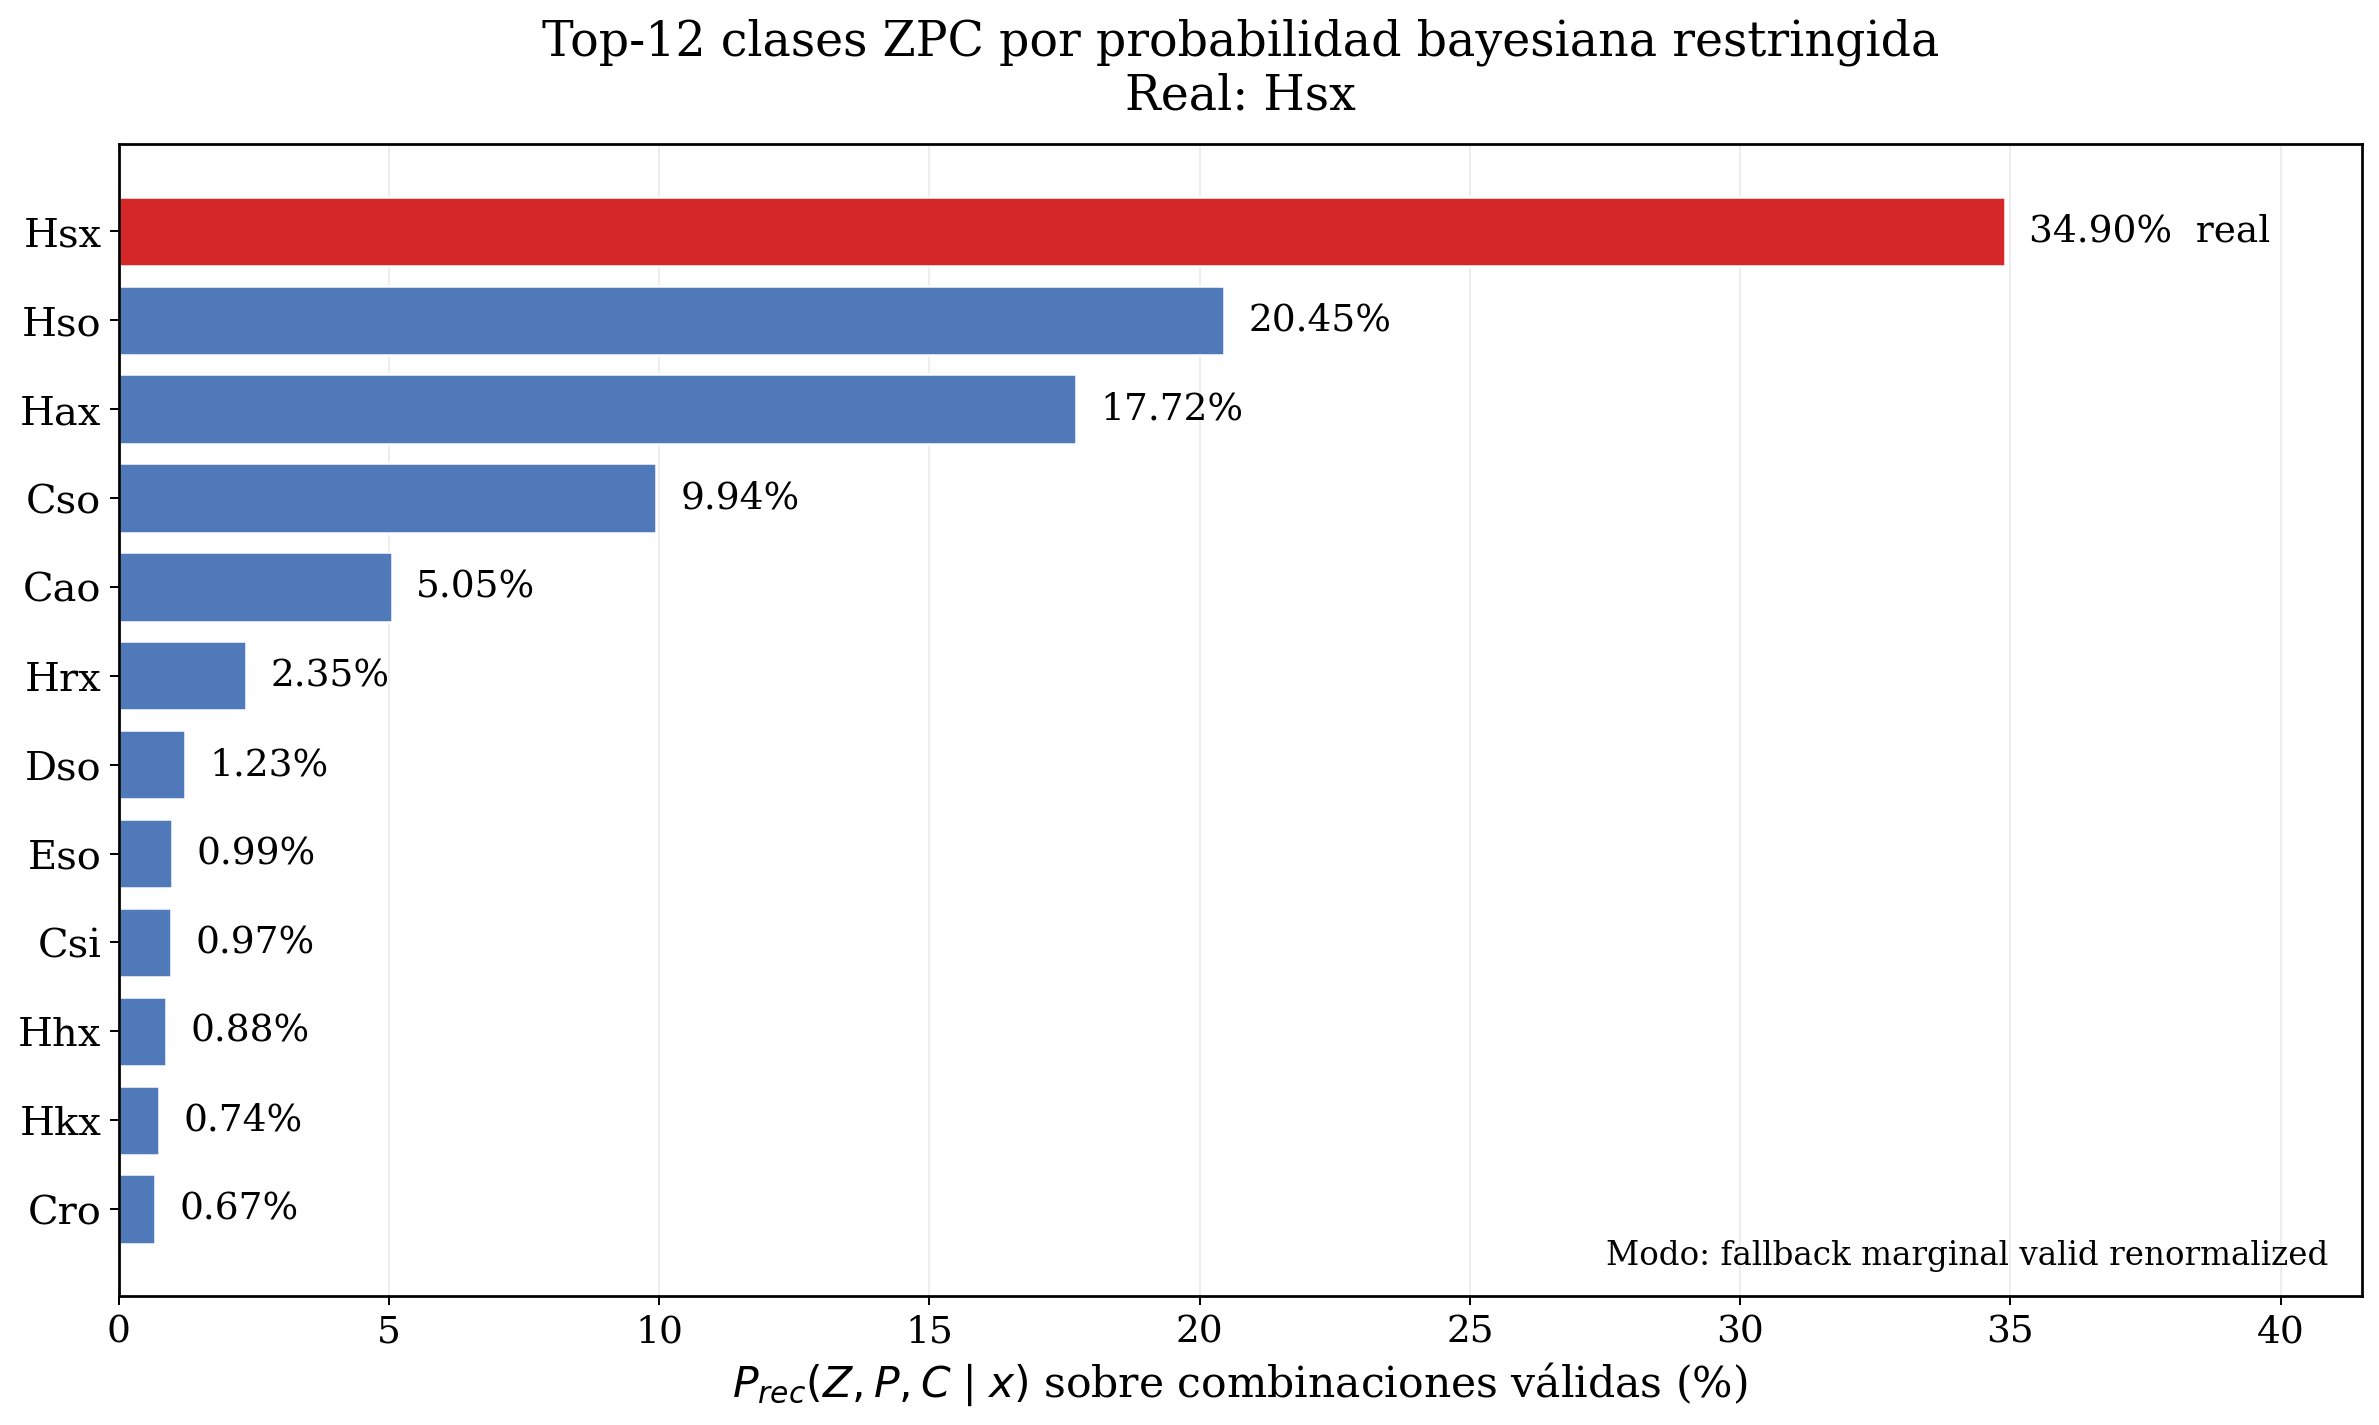
\includegraphics[width=0.92\linewidth]{figures/ml/top12_rec.png}
    \caption{Histograma de las doce clases Zurich--McIntosh con mayor probabilidad bayesiana restringida. \textbf{Fuente:} Elaboración propia.}
    \label{fig:resumen-top12-probabilidades}
\end{figure}

\begin{table}[H]
\centering
\caption{Comparación resumida de F1 por componente Zurich--McIntosh. \textbf{Fuente:} Elaboración propia a partir de los resultados del libro.}
\label{tab:resumen-f1}
%\scriptsize
\begin{tabular}{lcccc}
\toprule
\textbf{Modelo} & \textbf{$Z$} & \textbf{$P$} & \textbf{$C$} & \textbf{Prom.} \\
\midrule
Palladino et al. & 0.65 & 0.54 & 0.84 & 0.68 \\
Deng et al. & 0.47 & 0.41 & 0.60 & 0.49 \\
Propuesta & 0.65 & 0.63 & 0.71 & 0.66 \\
\bottomrule
\end{tabular}
\end{table}

Las métricas por clase permiten identificar cuáles componentes de la taxonomía presentan mayor ambigüedad. Para cada clase $c$, se emplean precisión, \textit{recall} y F1, definidos a partir de verdaderos positivos, falsos positivos y falsos negativos; esta lectura es necesaria porque el conjunto presenta desbalance y clases morfológicamente cercanas \citep{mcintosh1990classification,cui2019classbalanced,sayez2023sunscc}.

\begin{table}[H]
\centering
\caption{Métricas para salida $Z$. \textbf{Fuente:} Elaboración propia.}
\label{tab:resumen-metricas-z}
%\scriptsize
\begin{tabular}{lccc}
\toprule
\textbf{Clase} & \textbf{Precisión} & \textbf{Recall} & \textbf{F1} \\
\midrule
A & 0.79 & 0.73 & 0.76 \\
B & 0.74 & 0.71 & 0.72 \\
C & 0.68 & 0.61 & 0.64 \\
D & 0.63 & 0.61 & 0.62 \\
E & 0.49 & 0.39 & 0.43 \\
F & 0.47 & 0.39 & 0.43 \\
H & 0.78 & 0.84 & 0.81 \\
Prom. pond. & 0.68 & 0.63 & 0.65 \\
\bottomrule
\end{tabular}
\end{table}


\begin{table}[H]
\centering
\caption{Métricas para salida $P$. \textbf{Fuente:} Elaboración propia.}
\label{tab:resumen-metricas-p}
%\scriptsize
\begin{tabular}{lccc}
\toprule
\textbf{Clase} & \textbf{Precisión} & \textbf{Recall} & \textbf{F1} \\
\midrule
x & 0.57 & 0.31 & 0.40 \\
r & 0.34 & 0.28 & 0.31 \\
s & 0.59 & 0.63 & 0.61 \\
a & 0.46 & 0.54 & 0.50 \\
h & 0.71 & 0.65 & 0.68 \\
k & 0.84 & 0.82 & 0.83 \\
Prom. pond. & 0.66 & 0.61 & 0.63 \\
\bottomrule
\end{tabular}
\end{table}


\begin{table}[H]
\centering
\caption{Métricas para salida $C$. \textbf{Fuente:} Elaboración propia.}
\label{tab:resumen-metricas-c}
%\scriptsize
\begin{tabular}{lccc}
\toprule
\textbf{Clase} & \textbf{Precisión} & \textbf{Recall} & \textbf{F1} \\
\midrule
x & 0.62 & 0.52 & 0.57 \\
o & 0.46 & 0.47 & 0.46 \\
i & 0.79 & 0.72 & 0.75 \\
c & 0.82 & 0.84 & 0.83 \\
Prom. pond. & 0.74 & 0.69 & 0.71 \\
\bottomrule
\end{tabular}
\end{table}

Los modelos predictivos se evaluaron con métricas escalares y espacio-temporales. Para el SSN, el error absoluto medio ($\mathrm{MAE}$) mide el promedio de las desviaciones absolutas entre los valores reales y las estimaciones. La calidad del ajuste escalar también se resume mediante el coeficiente de determinación ($R^2$), el cual evalúa la proporción de la varianza explicada por el modelo respecto al promedio de la serie observada $\bar{z}$. 

Para la reconstrucción latitudinal se emplea el error relativo de Frobenius ($E_F$), diseñado para cuantificar la fidelidad global de la matriz reconstruida. Además, la coherencia espacio-temporal se mide con la correlación ($\rho_{ST}$) entre las matrices vec-transformadas, y el desvío medio del centro latitudinal se define a través del error de latitud central ($\mathrm{MLCE}$). Estas métricas distinguen entre precisión escalar y fidelidad de la migración latitudinal \citep{kalman1960newapproach,schmid2010dmd,kutz2016dmd}.

\begin{figure}[H]
    \centering
    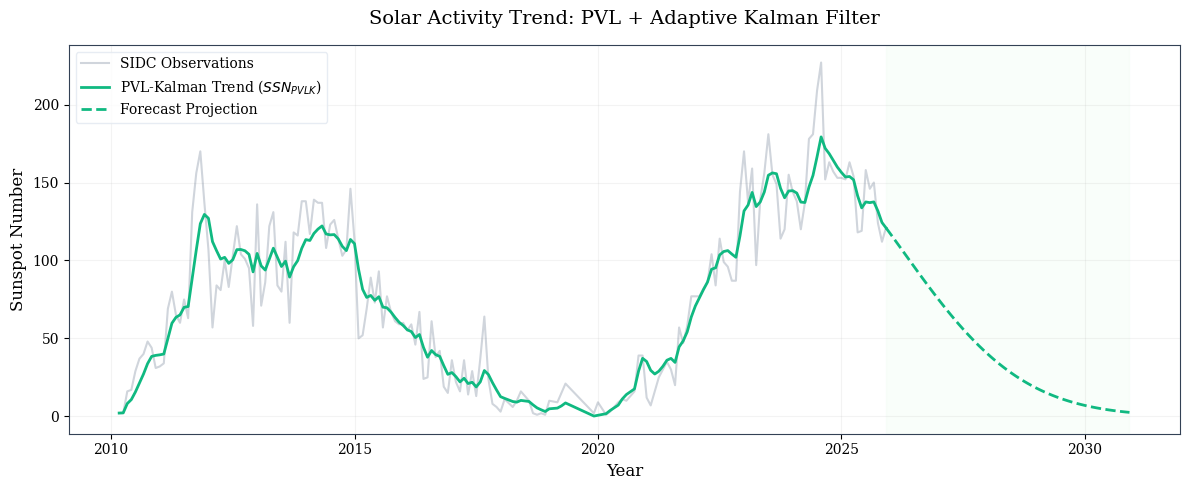
\includegraphics[width=0.92\linewidth]{figures/pred/kalman.png}
    \caption{Ajuste y predicción del número de manchas solares mediante PVL--Kalman. \textbf{Fuente:} Elaboración propia con base en el modelo PVL y el filtro de Kalman.}
    \label{fig:resumen-pvl-kalman}
\end{figure}

\begin{figure}[H]
    \centering
    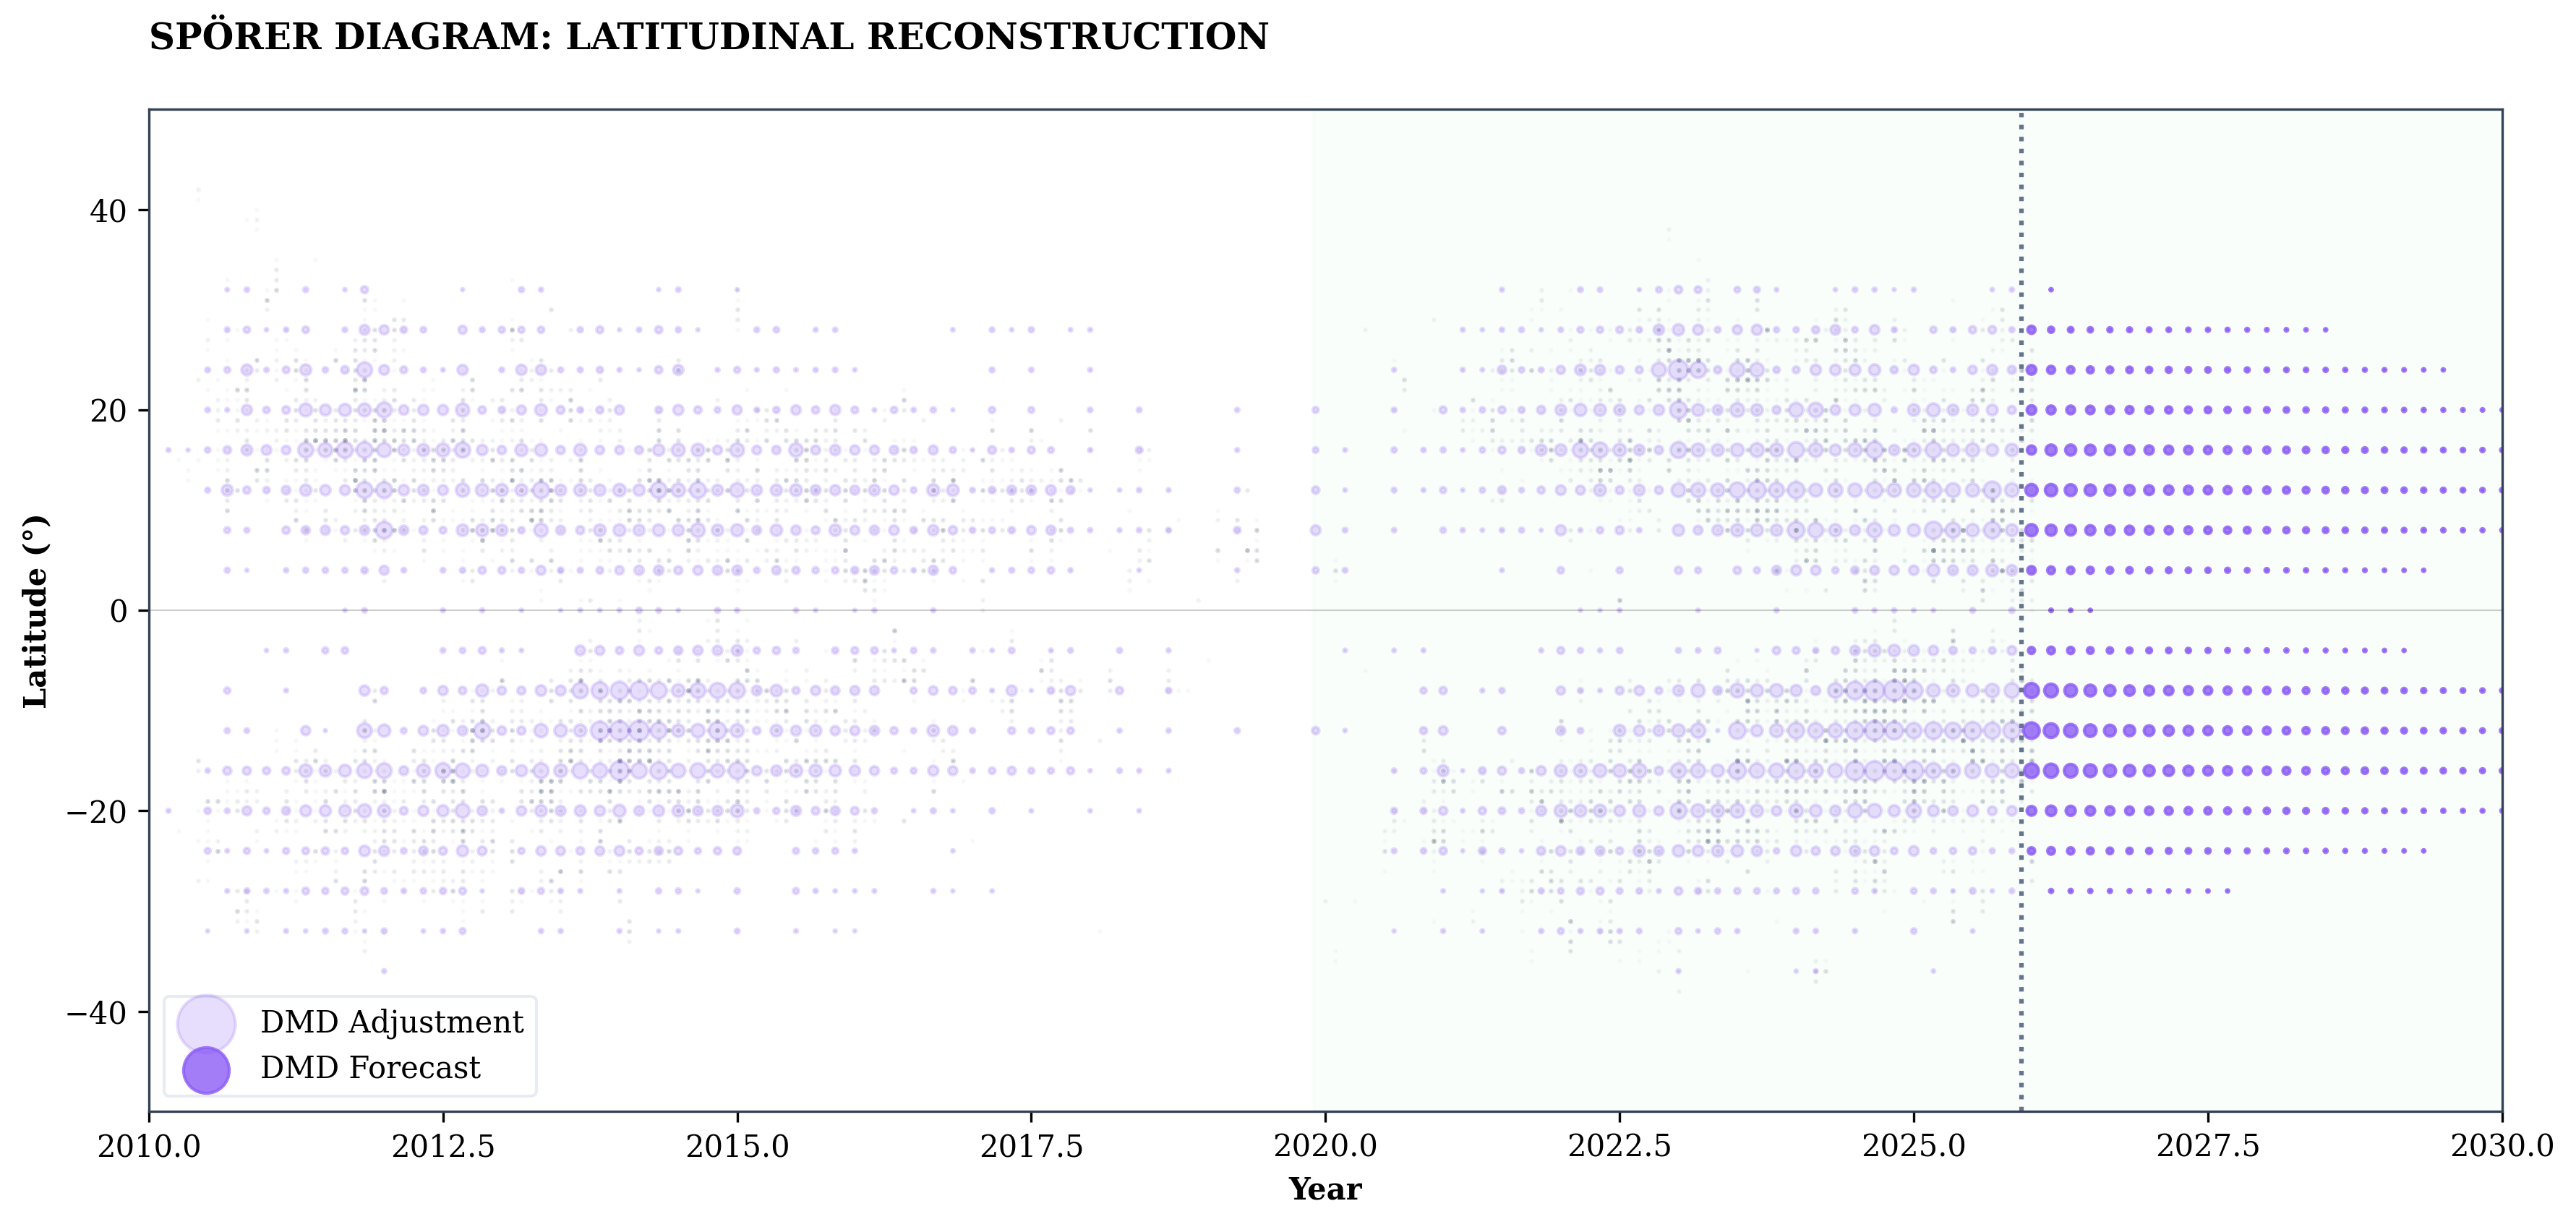
\includegraphics[width=0.92\linewidth]{figures/pred/sporer.png}
    \caption{Reconstrucción y predicción de la migración latitudinal de la actividad solar mediante DMD. La visualización conserva el patrón tipo diagrama de Spörer. \textbf{Fuente:} Elaboración propia.}
    \label{fig:resumen-sporer-dmd}
\end{figure}

\begin{figure}[H]
    \centering
    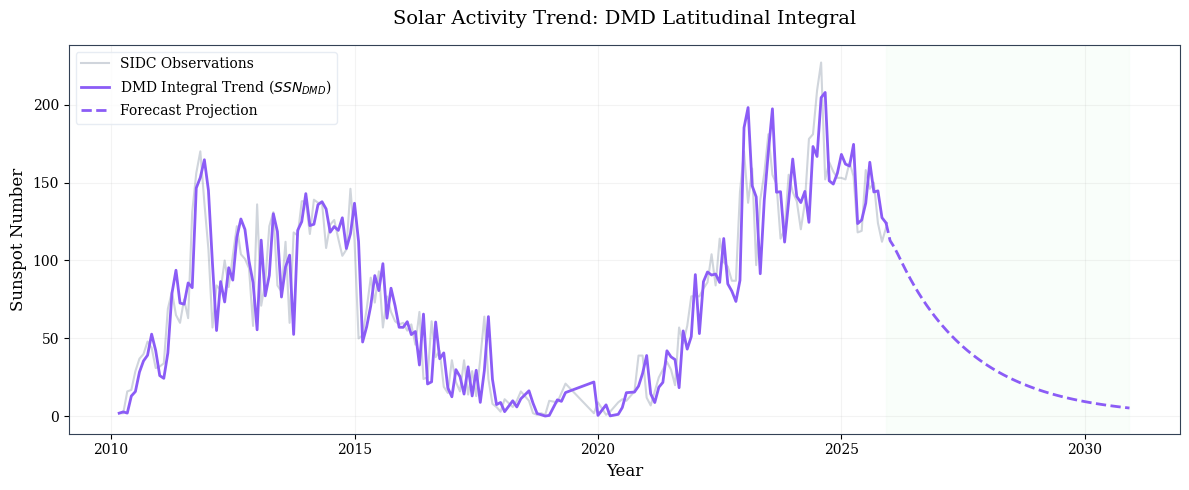
\includegraphics[width=0.92\linewidth]{figures/pred/dmd.png}
    \caption{Número de manchas solares derivado de la integral latitudinal del modelo DMD, $\mathrm{SSN}_{\mathrm{DMD}}(t)$. \textbf{Fuente:} Elaboración propia \citep{schmid2010dmd,kutz2016dmd}.}
    \label{fig:resumen-ssn-dmd}
\end{figure}

\begin{table}[H]
\centering
\caption{Métricas comparativas de validación predictiva para los modelos escalares SSN con ecuaciones de cálculo integradas. \textbf{Fuente:} Elaboración propia con base en los resultados experimentales.}
\label{tab:resumen-prediccion-escalar}
%\scriptsize
\begin{tabular}{lcc}
\toprule
\textbf{Métrica y Ecuación} & \textbf{$\text{SSN}_{\text{PVLK}}$} & \textbf{$\text{SSN}_{\text{DMD}}$} \\
\midrule
$\textstyle \mathrm{MAE}=\frac{1}{N}\sum_{k=1}^{N}|z_k-\widehat{s}_k|$ & 15.31 & 15.22 \\
\addlinespace
$\textstyle \mathrm{RMSE}=\sqrt{\frac{1}{N}\sum_{k=1}^{N}(z_k-\widehat{s}_k)^2}$ & 22.02 & 20.30 \\
\addlinespace
$\textstyle \mathrm{MAPE}=\frac{100}{N}\sum_{k=1}^{N}\left|\frac{z_k-\widehat{s}_k}{z_k}\right|$ & 33.27\% & 32.54\% \\
\addlinespace
$\textstyle R^2=1-\frac{\sum_{k=1}^{N}\left(z_k-\widehat{s}_k\right)^2}{\sum_{k=1}^{N}\left(z_k-\bar{z}\right)^2}$ & 0.8173 & 0.8449 \\
\bottomrule
\end{tabular}
\end{table}

\begin{table}[H]
\centering
\caption{Métricas de validación predictiva espacio-temporal para el modelo DMD-Spörer (Vectorial) con ecuaciones de cálculo integradas. \textbf{Fuente:} Elaboración propia con base en los resultados experimentales.}
\label{tab:resumen-prediccion-vectorial}
%\scriptsize
\begin{tabular}{lc}
\toprule
\textbf{Métrica y Ecuación} & \textbf{Valor} \\
\midrule
$\textstyle E_F=\frac{\|\mathbf{X}-\widehat{\mathbf{X}}\|_F}{\|\mathbf{X}\|_F}$ & 0.4087 \\
\addlinespace
$\textstyle \rho_{ST}=\mathrm{corr}\left(\mathrm{vec}(\mathbf{X}),\mathrm{vec}(\widehat{\mathbf{X}})\right)$ & 0.9126 \\
\addlinespace
$\textstyle \mathrm{MLCE}=\frac{1}{N}\sum_{k=1}^{N}|\theta_{c,k}-\widehat{\theta}_{c,k}|$ & 1.25$^\circ$ \\
\bottomrule
\end{tabular}
\end{table}

El modelo PVL--Kalman resulta más adecuado para seguir la amplitud global del ciclo solar, mientras que DMD aporta una salida no disponible en modelos unidimensionales: la distribución latitudinal y su migración hacia el ecuador. Por ello, ambos modelos se consideran complementarios dentro de la plataforma: uno sintetiza la evolución temporal del SSN y el otro conserva estructura espacial útil para interpretación científica \citep{hathaway2015solarcycle,podladchikova2012kalman,kutz2016dmd}.

\subsection{Validación integral del sistema}

La validación del hardware documentó el montaje de la cámara, la atenuación solar, la unidad de preprocesamiento y la integración con el telescopio. Además, una captura real realizada el 2026-05-05 permitió verificar adquisición, guardado local, preprocesamiento y sincronización con la base de datos bajo condiciones de operación de campo \citep{zwoASILinuxManual,raspberryPi5Docs2026}.

\begin{table}[H]
\centering
\caption{Métricas operativas representativas de la Raspberry Pi 5 durante la validación. \textbf{Fuente:} Elaboración propia.}
\label{tab:resumen-raspberry-operacion}
%\scriptsize
\begin{tabular}{lc}
\toprule
\textbf{Métrica} & \textbf{Valor representativo} \\
\midrule
Captura de imagen individual & 420 ms \\
Guardado local en microSD & 180 ms \\
Preprocesamiento básico por imagen & 1350 ms \\
Sincronización a Supabase & 3800 ms/imagen \\
Uso medio de CPU & 38\% \\
Uso máximo de CPU & 72\% \\
Uso de RAM del servicio local & 3.3 GB \\
Temperatura tras 25 min & 57 $^{\circ}$C \\
\bottomrule
\end{tabular}
\end{table}

Durante las pruebas no se observaron reinicios, cierres del servicio ni reducción térmica perceptible bajo refrigeración activa. Estos resultados respaldan la viabilidad del prototipo como nodo local de captura y asistencia, siempre que se mantenga ventilación adecuada y se considere la variabilidad de red durante la sincronización \citep{raspberryPi5Docs2026,nmcliHotspot2026}.

\begin{figure}[H]
    \centering
    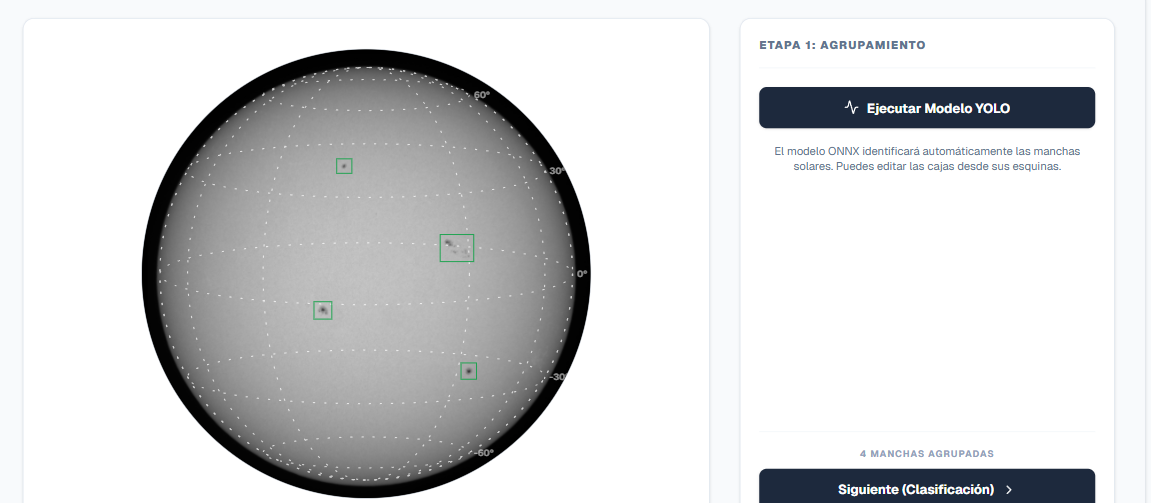
\includegraphics[width=0.9\linewidth]{figures/web/yolo.png}
    \caption{Validación de la etapa de agrupamiento \textit{on-device} mediante YOLO en la plataforma web. \textbf{Fuente:} Elaboración propia.}
    \label{fig:resumen-web-yolo-validacion}
\end{figure}

\begin{figure}[H]
    \centering
    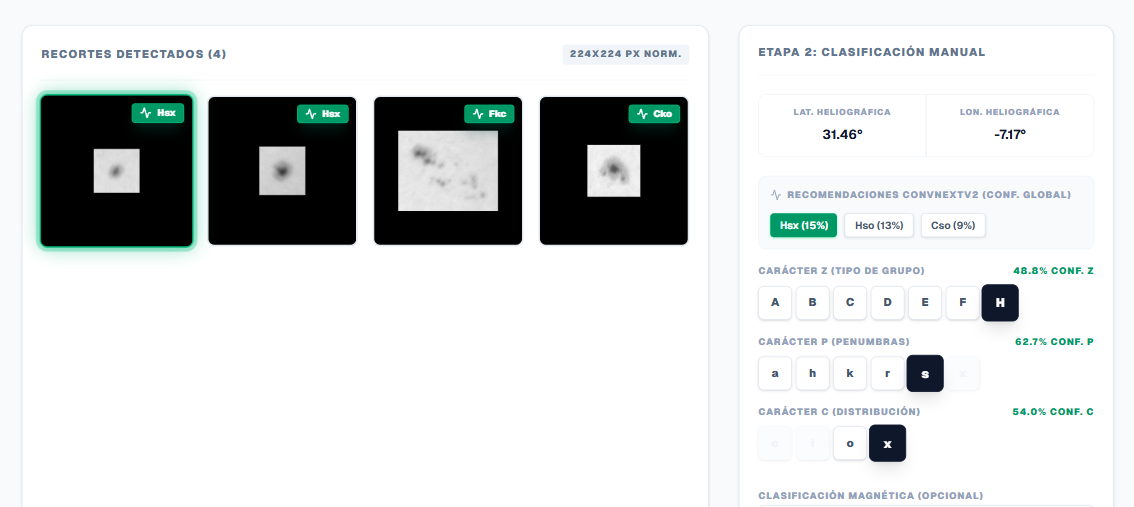
\includegraphics[width=0.9\linewidth]{figures/web/convnext.png}
    \caption{Validación de la etapa de clasificación morfológica \textit{on-device} mediante ConvNeXtV2 en la plataforma web. \textbf{Fuente:} Elaboración propia.}
    \label{fig:resumen-web-convnext-validacion}
\end{figure}

La plataforma web se validó mediante carga de modelos, consulta de datos desde Supabase e inferencia local en navegador; las Figuras~\ref{fig:resumen-web-yolo-validacion} y~\ref{fig:resumen-web-convnext-validacion} documentan, respectivamente, el agrupamiento con YOLO26n y la clasificación morfológica con ConvNeXtV2a. La ejecución se configuró con WebAssembly para aproximar el comportamiento en dispositivos sin aceleración GPU dedicada, verificando que los modelos ONNX pueden descargarse y ejecutarse como parte del flujo de asistencia observacional \citep{camporeale2019ml,ultralyticsYOLO26,woo2023convnextv2}.

\begin{table}[H]
\centering
\caption{Rendimiento resumido de la plataforma web durante la validación. \textbf{Fuente:} Elaboración propia.}
\label{tab:resumen-web-rendimiento}
%\scriptsize
\begin{tabular}{lc}
\toprule
\textbf{Métrica} & \textbf{Valor} \\
\midrule
Proveedor de ejecución & WASM \\
Tiempo de descarga del modelo & 5803 ms \\
Tiempo de galería Supabase & 1702 ms \\
Inferencia YOLO & 3105 ms \\
Inferencia de clasificación & 3201 ms \\
\bottomrule
\end{tabular}
\end{table}

\section{Discusión y conclusiones}

La principal contribución del trabajo no se limita al entrenamiento de un detector o un clasificador, sino a la construcción de una arquitectura coherente que conecta adquisición, metadatos, inferencia, visualización y análisis temporal. Esta integración conserva trazabilidad entre imagen original, recorte, predicción y consulta posterior, condición esencial para aplicaciones científicas y educativas \citep{scherrer2012hmi,noaaSRS,camporeale2019ml}.

El enfoque jerárquico resulta apropiado para la taxonomía Zurich--McIntosh porque respeta su estructura observacional y evita una clasificación plana de combinaciones. Sin embargo, el desbalance de clases, la ambigüedad morfológica y la dependencia de recortes bien localizados siguen siendo limitaciones relevantes para clases raras o configuraciones visualmente cercanas \citep{mcintosh1990classification,bornmann1994flarerates,cui2019classbalanced}.

La ejecución local y la conversión de modelos a ONNX refuerzan la portabilidad del sistema, especialmente en observatorios con conectividad limitada. Esta capacidad permite procesar cerca del punto de captura, reducir latencia y mantener consulta posterior mediante una plataforma web, sin depender completamente de infraestructura centralizada \citep{ultralyticsYOLO26,woo2023convnextv2,raspberryPi5Docs2026}.

Se concluye que el prototipo constituye una base funcional para observación solar asistida por inteligencia artificial en entornos académicos locales. Como trabajos futuros se propone ampliar campañas de validación, mejorar calibración y control de exposición, incorporar más datos propios, fortalecer la estimación heliográfica y refinar los modelos predictivos \citep{cesarHeliographic,podladchikova2012kalman,schmid2010dmd}.
\section{Agradecimientos}

Los autores agradecen al proyecto FEEI--CONACYT--PROCIENCIA ESTR01-23 ARASY, al programa de becas PUBIABM y al Observatorio Astronómico ``Prof.~Alexis Troche Boggino'' por el apoyo financiero, institucional y académico brindado a esta investigación.

Se reconoce el valor de los repositorios y catálogos públicos utilizados como referencia para datos solares, reportes observacionales y validación conceptual del sistema, especialmente los recursos asociados a observación heliográfica, reportes NOAA SRS e instrumentación solar abierta a la comunidad científica \citep{noaaSRS,scherrer2012hmi,bobra2014sharp,sidcGroundObservations2026}.

\section{Referencias}
\bibliographystyle{fiuna}
\bibliography{fiuna}

\section{Anexo}

El acceso a los recursos digitales del proyecto se organiza mediante códigos QR para facilitar la consulta de la plataforma web y del repositorio de desarrollo.

\begin{figure}[H]
    \centering
    
\includegraphics[width=0.52\linewidth]{figures/qr/web.png}
    \caption{Código QR para acceder a la plataforma web del sistema: \url{https://sunspot-page-app.vercel.app}. \textbf{Fuente:} Elaboración propia.}
    \label{fig:resumen-qr-web}
\end{figure}

\begin{figure}[H]
    \centering
    
\includegraphics[width=0.52\linewidth]{figures/qr/repo.png}
    \caption{Código QR para acceder al repositorio del proyecto completo y su documentación: \url{https://github.com/carlobeni/sunspot-page-app/tree/master}. \textbf{Fuente:} Elaboración propia.}
    \label{fig:resumen-qr-repo}
\end{figure}

\end{document}
